\thispagestyle{lichsutoanhocnone}
\pagestyle{lichsutoanhoc}
\graphicspath{{../lichsutoanhoc/pic2/}}
\everymath{\color{lichsutoanhoc}}
\blfootnote{$^1$\color{lichsutoanhoc}THPT chuyên Hà Nội -- Amsterdam.}
\begingroup
\AddToShipoutPicture*{\put(0,616){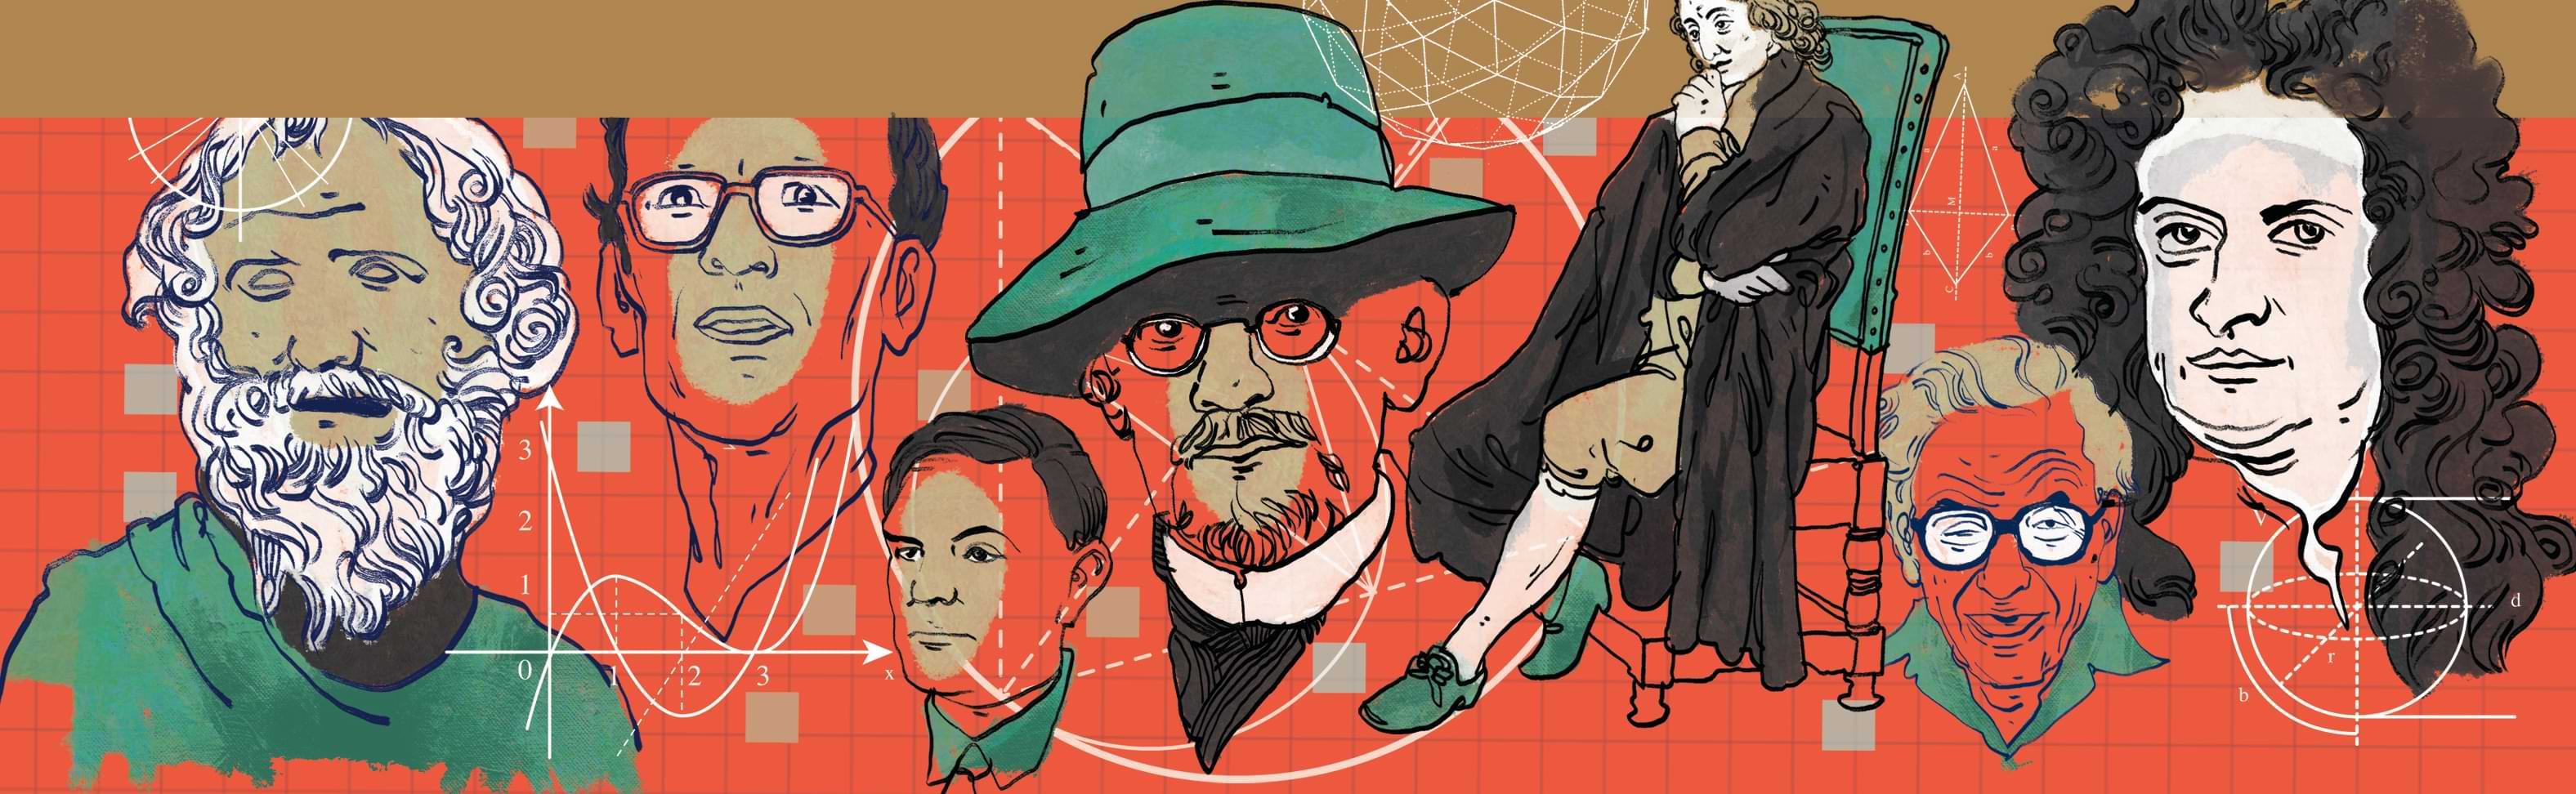
\includegraphics[width=19.3cm]{../bannerlichsu}}}
\AddToShipoutPicture*{\put(82,555){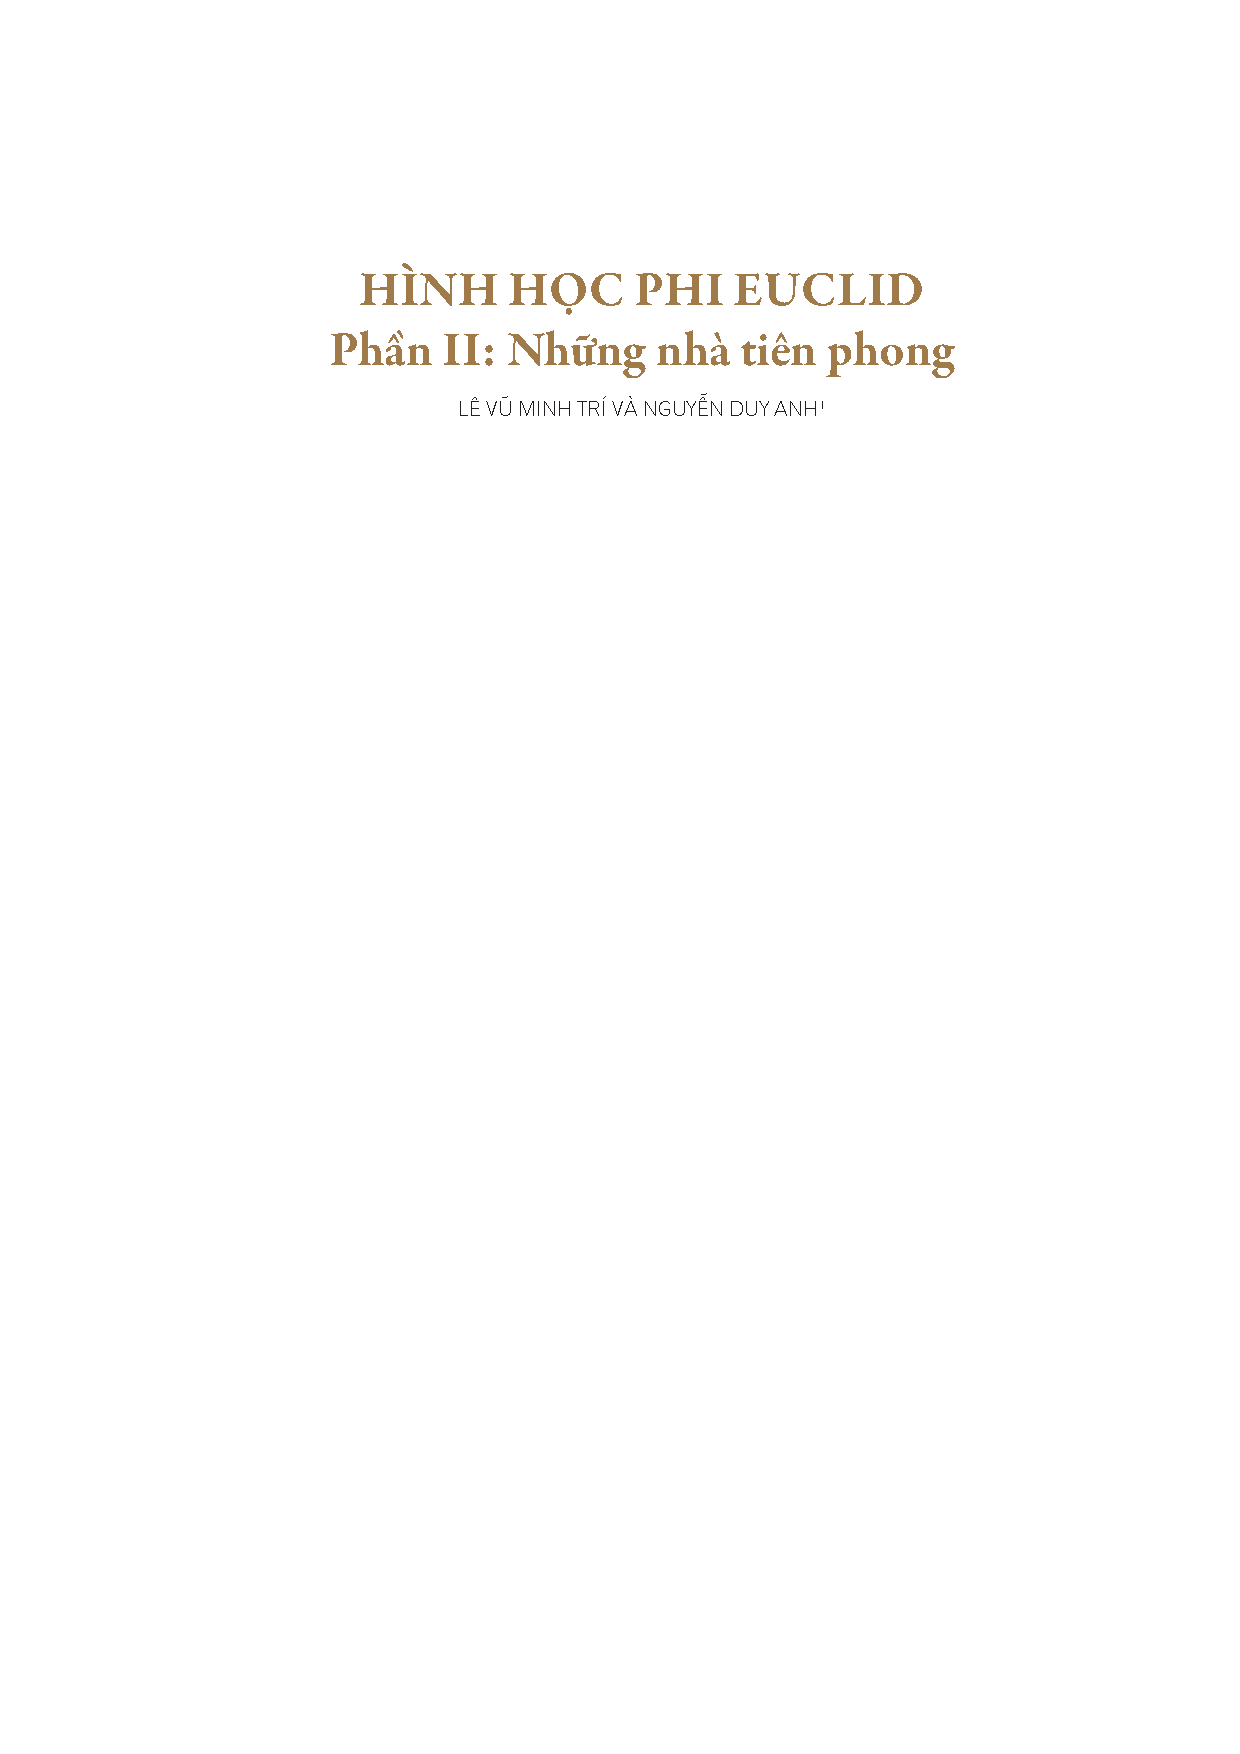
\includegraphics[scale=1]{../tieude3.pdf}}}
\centering
\endgroup

\vspace*{150pt}

\begin{multicols}{2}
	Một ý tưởng tưởng chừng như mâu thuẫn với những cảm quan thường thức, thế nhưng lại trở thành một vũ trụ hình học mới lạ và chặt chẽ, và có thể nắm giữ bản chất của không gian chúng ta đang sống. Thế nhưng quá trình khám phá và phát triển ý tưởng ấy phải trải qua hàng thập kỷ với nhiều trắc trở và gian nan.
	\vskip 0.1cm
	\textbf{\color{lichsutoanhoc}Những nhà tiên phong}
	\vskip 0.1cm
	Tiếc cho Saccheri khi tác phẩm giá trị của ông không nhận được sự chú ý của nhiều người hơn, vì thế nên câu hỏi về tiên đề $5$ của Euclid vẫn còn dai dẳng tới tận cả thế kỷ sau. Và số phận lần nữa lại trêu ngươi các nhà Toán học, khi mà không phải một, mà tận ba người đã gần như cùng lúc đến với đáp án cho câu hỏi lớn của chúng ta. Dù vậy, cách tiếp cận vấn đề của họ khác nhau một trời một vực.
	\vskip 0.1cm
	Carl Friedrich Gauss là một trong những nhà Toán học vĩ đại nhất mọi thời đại. Trong suốt chiều dài sự nghiệp, ông đã để lại những công trình vượt xa tri thức thời ấy trong rất nhiều lĩnh vực như lý thuyết số, lý thuyết xác suất, hình học và lý thuyết hàm số. Khác với những Leonhard Euler hay Augustin Louis Cauchy xuất bản vô cùng tích cực, Gauss tuân thủ triết lý ``Ít nhưng chín" (pauca sed matura): chỉ khi nào ông suy ngẫm đến mức đủ thấu đáo theo ý ông, và chỉ khi ông đã trình bày súc tích vấn đề ấy, ông mới cho đăng một nghiên cứu nào đó. Những ý tưởng ``chưa đủ chín" được ông tập hợp lại trong ngăn bàn làm việc, nơi mà dần dà tích trữ lượng tri thức đi trước thời đại $50$ năm. Khi Gauss bàn luận về Toán, thường sẽ có một tập giấy trong đó có ích cho cuộc trao đổi, được lấy ra sau câu cửa miệng ``tôi cũng đã suy nghĩ về vấn đề đó rồi", đôi lúc kèm theo ``tôi cũng đã đạt đến những kết quả tương tự".
	\vskip 0.1cm
	Không lĩnh vực Toán nào là Gauss không chạm tới, và câu hỏi về tiên đề thứ $5$ không phải ngoại lệ. Nhà Toán học vĩ đại đã trăn trở về vấn đề này từ năm lên $15$, và sau nhiều thất bại, ông dần nghi ngờ sự tồn tại của một chứng minh. Cũng như những người đi trước, ông đã thử giả sử phản chứng tiên đề $5$, cũng khám phá ra nhiều kết quả mà chưa thấy mâu thuẫn xuất hiện.Ông chưa vội xuất bản gì về những phát hiện ấy, mà tự mình tìm tòi trong đó cho đến khi bản thân ông đã hài lòng. Ngoài phương châm xuất bản của bản thân, còn một thế lực khác khiến ông dè dặt. Chả là có một người đồng hương đương thời có ảnh hưởng chẳng kém cạnh Gauss chút nào đã lên tiếng -- triết gia Immanuel Kant. Kant đồng ý rằng kiến thức bắt đầu từ những trải nghiệm từ bên ngoài, nhưng cho rằng trí óc có thể hành động dựa trên những ấn tượng chỉ có thể là bởi nó đã có những ``trực giác" về không gian và thời gian độc lập với kinh nghiệm, và cũng đúc khuôn những kinh nghiệm ấy. ``Khái niệm của không gian Euclid không có nguồn gốc thực nghiệm nào cả, mà là sự cần thiết không thể tránh khỏi của suy nghĩ. Không hệ thống hình học nào khác tồn tại, vì không hệ thống hình học nào khác có thể được hình dung.", Kant viết.
	\vskip 0.1cm
	Riêng khẳng định vừa rồi là sai, bởi các nhà Toán học đã hiểu được phần nào lời giải của vấn đề về tiên đề $5$, và sắp tới thì hi vọng là quý độc giả cũng vậy. Về phần Gauss, do sự đông đảo của các tín đồ theo Kant và những ``người hâm mộ" Euclid, ông tránh né gây hấn với họ, có nghĩa là ông không xuất bản các phát hiện của mình. Tất nhiên Gauss không chỉ có một mình, mà một bằng hữu của ông sẽ có đóng góp lớn vào các sự kiện sắp tới.
	\vskip 0.1cm
	Farkas Bolyai ($1775-1856$) là nhà toán học người Hungary, ban đầu học ở Jena, về sau trở thành đồng môn và một người bạn gần gũi của Gauss khi hai người học ở Gottingen. Mối quan hệ này được họ duy trì suốt phần đời còn lại. 
	\vskip 0.1cm
	Sau nhiều nỗ lực và tâm sức, Bolyai đã nhận ra một điều đáng chú ý về tiên đề song song: ông không thể chứng minh được nó mà không ngộ nhận. Có một lần người bạn Gauss còn giúp ông nhận ra sai sót của mình trong một chứng minh bất thành. Là một nhà toán học khá xuất sắc, với một tác phẩm nổi tiếng về Toán sơ cấp, Tentamen Juventutem Studiosam in Elementa Matheseos Purae (tạm dịch ``Nỗ Lực Giới Thiệu Những Yếu Tố của Toán Thuần Túy tới Thanh niên Ham học"), thế nhưng danh tiếng của Farkas Bolyai hầu như đến từ việc ông là \ldots cha của con ông, Janos Bolyai. Janos ($1802-1860$) từ sớm đã tỏ ra là một nhà toán học uyên bác hơn cả cha mình. Đơn cử như khi Farkas đổ bệnh, ông đã cho cậu con trai mới $13$ tuổi đứng lớp thay. Không muốn uổng phí tiềm năng của cậu quý tử, Bolyai cha đã gửi thư cho Gauss nhờ ông thu nhận Janos, nhưng oái oăm thế nào mà chẳng được hồi đáp sau tận $16$ năm. Vì thế chàng trai trẻ đã rẽ ngang sang học ở Viện Kỹ Thuật Hoàng Gia tại Vienna năm $1817$, và đi theo quân đội sau khi tốt nghiệp. Trong $10$ năm sau đó, Janos không chỉ là một nhà toán học sâu sắc, mà còn là một nghệ sĩ violin say mê, và một chuyên gia đấu kiếm. Cậu từng chấp nhận lời thách thức đấu kiếm với $13$ sĩ quan kỵ binh, với điều kiện là cậu được chơi violin sau mỗi $2$ trận đấu. Kết quả là $13-0$ cho Janos.
	\vskip 0.1cm
	May cho chúng ta, và ban đầu là không may lắm cho người cha Farkas, chàng thanh niên Janos tài năng cũng bị bài toán chứng minh tiên đề $5$ hớp hồn, rồi lao vào nghiên cứu. Cha cậu ngậm ngùi nhớ lại kết cục ông từng trải, nhắn gửi cậu những lời sau đây:
	\vskip 0.1cm
	``Đừng dành một giờ đồng hồ nào cho vấn đề đó (tiên đề song song). Nó không đưa đến một kết quả nào cả; thay vào đó nó sẽ đầu độc cả cuộc đời con \ldots Ta tin rằng bản thân ta đã tìm ra mọi ý tưởng có thể nghĩ tới liên quan đến vấn đề này."
	\vskip 0.1cm
	Trái với mong muốn của cha, Janos được tiếp thêm động lực để tiếp tục, nhưng rồi chuỗi bất bại $2000$ năm của bài toán ấy cũng dần khiến cậu nghĩ rằng tiên đề số $5$ thực sự không phải định lý. Và cậu cũng chọn đi con đường giả sử phản chứng, tiếp tục đào sâu vào thứ Hình học xa lạ giờ đây đang dần được cậu định hình rõ nét. Khác với Saccheri, cậu chẳng vướng bận với nghĩa vụ chứng minh Euclid là đúng; trong mắt chàng trai trẻ, thế giới mới này rực rỡ chẳng kém gì thứ hình học được tôn sùng bấy lâu. Thành quả của cậu khiến chính người cha thay đổi quan niệm. ``Từ hư không, con đã tạo ra một vũ trụ lạ lẫm và mới mẻ", Janos khẳng định trong một bức thư trao đổi với cha. 
	\vskip 0.1cm
	Farkas hí hửng thêm những kết quả ấy vào trong cuốn ``Tentamen" lần tái bản năm $1832$, dưới tiêu đề Appendix Scientiam Spatii Absolute Veram Exhibens (Phụ lục Giải thích Khoa học Tuyệt đối của Không gian), đồng thời nối lại liên lạc với cây đa cây đề Gauss của Toán học đương thời. Gauss hết lời tán dương, song lại có đoạn ông viết:
	\vskip 0.1cm
	``Nếu tôi bắt đầu với việc nói rằng tôi không dám khen ngợi công trình này, hẳn trong một khắc anh sẽ ngạc nhiên, nhưng tôi không thể làm khác. Khen ngợi nó đồng nghĩa với việc khen ngợi chính tôi. Vì toàn bộ nội dung của công trình, từ cả hướng tiếp cận của con trai anh, tới cả những kết quả mà nó thu được, trùng khớp gần như hoàn toàn những suy nghĩ đã chiếm giữ đầu óc tôi suốt ba mươi hay ba mươi lăm năm qua \ldots Kế hoạch của tôi là viết tất cả ra giấy, để ít nhất thì những ý tưởng này không theo tôi xuống mồ. Nên tôi rất ngạc nhiên khi có người đã làm việc này thay tôi, và đặc biệt vui mừng khi người đó lại chính là con trai của người bạn cũ đã vượt xa tôi một cách ấn tượng đến vậy."
	\vskip 0.1cm
	Câu cuối với Janos như là Gauss khẳng định ông lấy cắp ý tưởng của cậu. Thật ra, những kết quả cậu (và nhân vật thứ ba mà chúng ta sắp nói đến) đạt được chi tiết và phong phú hơn Gauss rất nhiều, điều này chính Gauss còn công nhận. Vốn tính khí nóng nảy, cậu trai thất vọng kinh khủng, và khoảnh khắc ấy là lúc cậu đoạn tuyệt với xuất bản (hên cho hậu thế là khoảng $20000$ trang bản thảo của Janos vẫn còn). Dù về sau đã dẹp bỏ được mối nghi ngờ về nhà Toán học lão thành, Janos vẫn chẳng thể vực dậy tinh thần bản thân do công trình của cậu chẳng hề được người đời hưởng ứng. Đạp đổ một tượng đài trong lòng nhân loại suốt hai thiên nhiên kỷ chẳng phải dễ dàng, và điều ấy càng khắc sâu nỗi thất vọng vốn có. Sự công nhận xứng đáng cho Janos đáng tiếc lại không đến khi cậu còn sống.
	\vskip 0.1cm
	Quay ngược thời gian về năm $1829$, $3$ năm trước bài báo của Janos, một bài báo về chủ đề tương tự đã xuất hiện tại nước Nga xa xôi. Tác giả là nhân vật chính thứ ba, Nikolai Lobachevsky. 
	\vskip 0.1cm
	Nói qua về bối cảnh giáo dục Nga thời ấy. Giáo dục nói chung và Toán học nói riêng ở Nga giai đoạn cuối thế kỷ $18$ -- đầu thế kỷ $19$ chưa được phát triển như các quốc gia phương Tây khác. Tình hình không khả quan hơn sau khi cuộc chinh phạt của Napoleon đại đế sa lầy giữa mùa đông nước Nga, bởi sự kiện này đã làm dậy lên hai hiện tượng trong lòng người dân Nga thời bấy giờ: họ dần có ác cảm với những ảnh hưởng ngoại bang, và niềm tin vào một Đấng tối cao thần bí cứu rỗi mẫu quốc Nga vĩ đại được nhen nhóm lại mạnh mẽ, không tốt cho phát triển khoa học. Đứng trước hai cơn gió ngược chiều, công cuộc cường hóa nền giáo dục nước nhà, lấy ấy làm tiềm lực quốc gia của Sa Hoàng Aleksandr chẳng hề thuận lợi. Lobachevsky đến tuổi vào Đại học Kazan trong bối cảnh đó, và sẽ dành $40$ năm cuộc đời ông gắn bó với nơi đây.
	\vskip 0.01cm
	Chẳng rõ tự bao giờ, Lobachevsky đã nghiền ngẫm và thử đưa ra những chứng minh, cũng đã nghi ngờ và thử giả sử mệnh đề phủ định của tiên đề song song, và cũng đã theo mạch phát triển mà chẳng thấy mâu thuẫn nào. Đến lúc ấy, hẳn Lobachevsky đã bị thuyết phục bởi lượng kết quả mới quá nhiều để có thể dẫn đến một mâu thuẫn, ông dành tận $3$ năm phát triển hệ thống ông mới tạo dựng. Ông cho xuất bản những kết quả của mình trên tờ ``Messenger" của Kazan, và chỉ nhận lại cái quay lưng lạnh nhạt của giới học thuật. Ngoài việc nền giáo dục Nga xa cách với các trung tâm sôi nổi của cộng đồng nghiên cứu, điều này một phần còn do Lobachevsky đặt tên loại hình học này là ``hình học tưởng tượng" (imaginary geometry). Bài báo ``Về Nền tảng của Hình học" của ông còn bị từ chối bởi một reviewer thờ ơ thuộc Viện Hàn lâm Khoa học St. Petersburg, với lý do hai tích phân xác định trong bài báo thì một cái là sai, cái còn lại thì dễ chứng minh. Sở dĩ một bài báo về hình học có yếu tố giải tích là bởi Lobachevsky đã phát triển lượng giác của loại hình học này.
	\end{multicols}
	\begin{multicols}{2}
	Lobachevsky không vì phản ứng của dư luận mà nhụt chí. Ông ra sức viết hàng loạt bài báo để thuyết phục giới học thuật về tầm cỡ của thành tựu của ông. Ông vẫn hết mình với ngôi trường ông giảng dạy, hết mình với lao động. Khi trao đổi những kết quả với Gauss, ông nhận lại những lời khen có cánh, thậm chí là lời đề nghị ông giữ một chân tại khoa Toán Đại học Gottingen cạnh Gauss. Lobachevsky từ chối. Trong suốt những năm tháng gắn bó với Đại học Kazan, Lobachevsky đã kiêm vai trò của giảng viên, nhà nghiên cứu, thành viên hội đồng quản trị, lao công, thậm chí từng thiết kế kiến trúc và giúp trường chống dịch tả.
	\vskip 0.1cm
	Đáp lại những công lao đó, trung ương đã hào phóng tặng một Lobachevsky đã ngoài ngũ tuần một lượt về hưu non. Có người cho rằng, những thế lực khiến Gauss e ngịa đã nhúng tay vào: những tín đồ của Euclid và Kant hẳn đã rỉ tai gia đình hoàng tộc về thứ hình học mới đã xúc phạm đến tượng đài tri thức của  Hy Lạp và Euclid. Kể cả quyết định đột ngột trên, hay nỗi đau mất con, hay sự mù lòa sau này, tất cả vẫn chẳng thể quật ngã Lobachevsky, ông vẫn nghiên cứu về loại hình học phủ định tiên đề song song chừng nào ông còn nghĩ được, vẫn nhiều lần xuất bản thêm đến cuối đời. Vào kỷ niệm $50$ năm thành lập Đại học Kazan, ông lại cho đăng tải một bài báo về công trình để đời ông, lúc này được ông gọi là Pangeometry. Đổi tên vẫn không giúp ông nhận được sự công nhận xứng đáng.
	\vskip 0.1cm
	Cùng một bài toán ta có ba cách tiếp cận: người thì giữ làm bí mật do lo sợ thời thế, người lại cay đắng thất vọng sau một bức thư, người lại chẳng hề ngán bất cứ điều gì, vững tin vào thành quả bản thân. Dù gì đi nữa thì những công trình quá sức công phu để bị bác bỏ của họ đã khiến dư luận dần có lý do để tin:
	\vskip 0.1cm
	\textit{Tiên đề song song không thể được chứng minh từ các tiên đề còn lại} 
	\vskip 0.1cm
	$\pmb{2.}$ \textbf{\color{lichsutoanhoc}Sự phi mâu thuẫn}
	\vskip 0.1cm
	Tuy nhiên có một điều cả $3$ người tiên phong trên thiếu. Loại hình học họ nghĩ ra vẫn thuần túy ``nằm trên giấy", sự phi mâu thuẫn của nó vẫn chỉ là giả định. Hình dung hậu thế dốc sức phát triển hàng trăm định lý, để rồi ai đó phát hiện ra một mâu thuẫn quá đỗi đơn giản nào đó. Mà từ các mệnh đề mâu thuẫn, người ta có thể chứng minh được mọi mệnh đề, nên một hệ tiên đề chứa mâu thuẫn chắc chắn là không đem lại giá trị gì. Nhiệm vụ cấp thiết tiếp theo chính là chứng minh sự phi mâu thuẫn đó.
	\vskip 0.1cm
	Mọi nghi ngờ cuối cùng cũng được giải quyết bởi Eugenio Beltrami ($1835-1900$) vào năm $1868$ (người đàn ông này cũng giới thiệu lại công trình bị bỏ quên của Saccheri): hình học Euclid và loại hình học mới mẻ này ``đúng như nhau". 
	\vskip 0.1cm
	Cách làm rất đơn giản: dựng ra một không gian tuân theo quy luật của hình học mới trong chính không gian của hình Euclid. Và mô hình mà Beltrami lựa chọn là bề mặt của một ``ngụy cầu" (pseudosphere), thứ mà ta thu được khi ta quay một đường cong tractrix xung quanh trục hoành. Nếu định nghĩa đường thẳng trên bề mặt này là đường đi ngắn nhất giữa $2$ điểm, thì một phần các tính chất hình học trên bề mặt này thỏa mãn hình học của Bolyai và Lobachevsky. 
	\vskip 0.1cm
	Quan trọng hơn, mọi định lý của loại hình học trên bề mặt này có thể được quy về một định lý tương ứng trong hình học Euclid, tức là nếu hình học mới này có mâu thuẫn, thì hình học của Euclid cũng vậy. Nói cách khác, hình học Euclid, thứ ở vị trí thống trị suốt từ thời Hy Lạp cổ đại đến lúc ấy, chỉ ``đúng ngang với" hình học mới của Gauss, Bolyai và Lobachevsky mà thôi. Phần phân tích hai mô hình Beltrami--Klein và Poincaré sẽ chứng minh điều này ở mức độ hình học sơ cấp hơn.
	\vskip 0.1cm
	Lúc này ta càng phải trân trọng sự thiên tài của Euclid. Ông không những xếp đây là tiên đề sau cùng, mà còn hoãn việc dùng đến nó trong tận $29$ kết quả đầu tiên trong ``Elements". Những gì mà tận hai thiên niên kỷ sau mới phát hiện là bảo chứng cho tính độc lập của tiên đề thứ $5$: nó không thể là một định lý rút ra từ chỉ $4$ tiên đề đầu tiên. Tiên đề thứ $5$ thật sự là một tiên đề độc lập.
	\vskip 0.1cm
	Lộn lại vấn đề về gốc rễ, xét mệnh đề phủ định của tiên đề $5$ theo phát biểu của Playfair:
	\vskip 0.1cm
	Tiên đề $5$: Cho trước $1$ điểm $M$ không nằm trên $d$, có đúng một đường thẳng $d'$ đi qua $M$ và song song với $d$
	\vskip 0.1cm
	sẽ có phủ định là: 
	\vskip 0.1cm
	Tồn tại một điểm $M$ và đường thẳng $d$ không đi qua nó, sao cho số đường thẳng đi qua $M$ và song song với $d$ là khác $1$. Con số này có thể là $0$ hoặc ít nhất $2$. 
	\vskip 0.1cm
	Hóa ra, trường hợp thứ hai tương đương với giả thuyết góc nhọn vững chãi mà Saccheri đã không loại được. Còn trường hợp con số ấy là $0$, nói cách khác là mọi đường thẳng đều giao nhau, thì vị tu sĩ của chúng ta đã loại ngon ơ rồi mà. 
	Bước tiến tiếp theo sau đây sẽ giải đáp được điều ẩn khuất sau trường hợp bị loại đó và rất nhiều khúc mắc khác, cũng như gợi ra rất nhiều hướng đi mới cho Toán học và Vật lý thời kỳ tiếp theo.  
	\vskip 0.1cm
	$10/6/1854$, Gottingen. Trong căn phòng nơi bài Habilitation lecture diễn ra, hầu hết các thính giả đều không hiểu gì mấy, thậm chí cả trưởng khoa Toán ngồi nghe còn có phần lúng túng. Bài nói chuyện là về Hình học, nhưng trên bảng không có lấy một hình vẽ nào. Phải đến $10$ năm sau giới Toán học mới dần vỡ ra ý nghĩa của những gì diễn ra ngày hôm ấy: đến tận $1868$ những nội dung được bàn luận mới được xuất bản. Riêng việc vượt xa kỳ vọng của trưởng khoa Gauss thôi đã chứng thực cho sự kỳ tài của giảng viên trẻ Bernhard Riemann rồi.
	\vskip 0.1cm
	\textbf{\color{lichsutoanhoc}Đột phá}
	\vskip 0.1cm
	Bài nói chuyện gồm có hai phần.
	Trong phần đầu, Riemann đặt vấn đề định nghĩa không gian n-chiều (nay chúng ta gọi là không gian Riemann), trong đấy có những đường ngắn nhất gọi là đường trắc địa (geodesic lines), giống như những đường thẳng trong không gian Euclid. Từ đó định ra hệ tọa độ trắc địa và một metric cho những mặt cong nhiều chiều, theo cách mà chúng ta hình dung những mặt phẳng tiếp xúc với mặt cong trong không gian Euclid. Rồi thì trên những mặt cong ấy sẽ xác định những độ cong dương, âm, hoặc bằng không.
	Trong phần thứ hai, Riemann đặt vấn đề về sự liên hệ giữa hình học và thế giới chúng ta sống. Ông hỏi rằng chiều của thế giới thật sự trong đó chúng ta sống là bao nhiêu và hình học nào có thể dùng để mô tả thế giới ấy?
	\vskip 0.1cm
	Chúng ta sẽ đi qua vài ý tưởng mới mẻ của Riemann: khá niệm đa tạp, tổng quát hóa của khái niệm khoảng cách, và khái niệm độ cong. 
	\vskip 0.1cm
	Một đa tạp là tập các bộ $n$ số có sắp thứ tự $(x_1, x_2, \ldots, x_n)$. Sắp thứ tự nghĩa đơn giản là thứ tự viết các số có quan trọng, như là $(1, 2)$ thì khác $(2, 1)$ vậy. Số $n$ ở đây là số chiều của đa tạp. Từ việc nghĩ thông qua khái niệm này, khái niệm ``không gian" không bắt buộc phải được minh họa bởi một thực thể hữu hình nhất định nào đó, với các nhà toán học hiện đại, nó đơn giản là một loại đa tạp như ta minh họa ở trên thôi. 
	\vskip 0.1cm
	Để giải thích khái niệm độ cong, trước tiên xét các đường trên mặt phẳng Euclid. Hai hình một chiều cơ bản nhất của không gian Euclid là đường thẳng và đường tròn. Về mặt cảm nhận, ta sẽ muốn thiết lập để độ cong của một đường thẳng là $0$, nên quy ước đường thẳng có độ cong $k = 0$. Việc độ cong của một đường tròn phụ thuộc vào bán kính của nó cũng là dễ hiểu. Xét một điểm $P$ trên đường thẳng $l$. Vẽ một đường tròn bán kính $r$ tiếp xúc với $l$ tại $P$. Ta thấy khi $r$ càng tăng lên thì khu vực quanh đường tròn đó tại $P$ cong ngày càng chậm và trông ngày càng giống đường thẳng $l$. Do đó đặt độ cong của một đường tròn bán kính $r$ là $k = \frac{1}{r}$ là chuyện tự nhiên. Để ý rằng mọi điểm trên đường tròn có cùng độ cong, tức là đường tròn có độ cong là hằng số.
	\vskip 0.1cm
	Giờ ta xét một đường cong gamma đủ trơn bất kỳ trên $R^2$. Với mỗi điểm $P$, ta lấy một điểm $Q$ nào đó trên gamma và cho tiến dần về $P$, giới hạn của đường thẳng $PQ$ khi $Q$ tiến tới $P$ được gọi là tiếp tuyến của đường cong tại $P$. Tương tự khi cho hai điểm $Q, R$ tiến dần về $P$, $(PQR)$ sẽ có giới hạn, gọi là đường tròn mật tiếp (osculating circle) của gamma tại $P$. Về mặt trực giác, đường tròn này sẽ xấp xỉ tốt nhất (best fit) gamma tại gần $P$, do vậy có thể định nghĩa độ cong của gamma tại $P$ là độ cong của đường tròn đó, tức là $ \frac{1}{r}$. Do đường tròn ở các điểm có thể nằm về hai phía khác nhau của đường cong, chúng ta sẽ thay đổi định nghĩa một chút để thể hiện vị trí tương đối của chúng với gamma: đường tròn mật tiếp bán kính $r$ thì độ cong $ \frac{1}{r}$ hoặc $ \frac{-1}{r}$. Khi bán kính của đường tròn mật tiếp của các điểm dọc gamma biến đổi liên tục từ âm sang dương hoặc ngược lại, sẽ tồn tại một điểm trên gamma mà đường tròn mật tiếp suy biến thành đường thẳng.
	\vskip 0.1cm
	Những gì ta đã nói ở trên về các đường cong trên mặt phẳng thì cũng tương tự với một đường cong bất kỳ trong không gian, với một vài chỉnh sửa sau đây:
	\vskip 0.1cm
	Đường tròn mật tiếp khi này nằm trên một mặt phẳng Pi gọi là mặt phẳng mật tiếp (osculating plane) (trừ khi nó suy biến thành tiếp tuyến). Độ cong tại điểm $P$ được tính như sau: đặt $k$ là vectơ độ cong nằm trên mặt phẳng mật tiếp, có gốc là điểm $P$, vuông góc với tiếp tuyến tại $P$, có độ lớn $ \frac{1}{r}$, và hướng về tâm đường tròn mật tiếp (gọi là tâm độ cong). Nếu đường cong gamma có độ cong ở $P$ là $0$, thì $k$ là vectơ $0$. 
	\vskip 0.1cm
	Giờ ta đến một bề mặt $S$ trên $R^3$ (không gian). Ở một điểm bất kỳ trên bề mặt, tồn tại $2$ vectơ đơn vị vuông góc với mặt phẳng tiếp tuyến $T$ tại đó và ngược hướng nhau. Ở một lân cận bất kì trên mặt phẳng thì sẽ tồn tại hai trường liên tục các vectơ như vậy. Chọn một trong hai trường là dương sẽ định hướng lân cận đó. Nếu có một trường vectơ như vậy tồn tại trên toàn $S$, thì mặt phẳng $S$ được gọi là định hướng được. 
	\vskip 0.1cm
	Ví dụ minh họa cho dễ hiểu: Một mặt phẳng thông thường là định hướng được; có thể chọn $1$ trong $2$ mặt là mặt dương; một dải Mobius là một bề mặt không định hướng được.
	\vskip 0.1cm
	Giả sử $S$ có thể định hướng được. Nếu gamma là một đường cong trên $S$, thì ở mỗi điểm $P$ trên gamma ta có thể định nghĩa một độ cong đại số $k$. $k$ dương hay âm phụ thuộc vào việc tâm độ cong tại $P$ nằm ở phía dương hay phía âm của $S$.
	\vskip 0.1cm
	Gọi đường thẳng đi qua $P$, vuông góc với mặt phẳng tiếp tuyến tại $P$ là $T$. Xét một mặt phẳng chứa $T$ nào đó. Giao tuyến của mặt phẳng đó với $S$ là một đường cong (nằm trên mặt). Mỗi đường cong này có một độ cong khác nhau tại điểm $P$. Euler đã chứng minh những độ cong khác nhau này có giá trị lớn nhất $k_1$ và giá trị nhỏ nhất $k_2$. Hai đường cong tương ứng với hai giá trị này được gọi là các đường cong chính (principle curve), và Euler chứng minh được hai đường cong chính sẽ vuông góc với nhau nếu chúng phân biệt. Tích $K = k_1.k_2$ được gọi là độ cong Gauss. 
	\vskip 0.1cm
	Gauss đã chứng minh được rằng độ cong Gauss $K$ không thay đổi khi các bề mặt bị ``bẻ cong", miễn là sự bẻ cong ấy không thay đổi độ dài địa phương của cung và góc của những đường cong trên bề mặt ấy. 
	\vskip 0.1cm
	Ông phấn khích với kết quả này tới nỗi ông đặt tên cho nó là ``theorema egregium", tạm dịch là ``định lý phi thường". Gauss cũng tìm ra cách tính độ cong đại số của một bề mặt mà không dùng đến không gian ba chiều. Tưởng tượng một sinh vật $2$D nào đó sống trên một bề mặt, và không có ý niệm gì về chiều thứ $3$. Sinh vật này sẽ tính $K$ như thế nào? Để trả lời câu hỏi đó, ta sẽ đi qua khái niệm về khoảng cách Riemann đã tổng quát
	\vskip 0.1cm
	Điều mới mẻ Riemann đem lại là ``khoảng cách" giữa hai điểm trên một bề mặt bất kỳ không nhất thiết tuân thủ công thức ta quen biết. Ấy là, trong hệ trục tọa độ Oxy, theo định lý Pytago, khoảng cách giữa $2$ điểm $A(x, y)$ và $B(x + dx, y + dy)$ là:
	\begin{align*}
		AB = ds = \sqrt{dx ^2 + dy^2}.
	\end{align*} 
	Nếu độc giả còn nhớ, định lý Pytago thực chất lại chính là một tương đương của tiên đề $5$! Vì thế trong những loại hình học mà tiên đề $5$ không đúng, thì quy ước khoảng cách này không hợp lý. Với mỗi không gian khác không gian Euclid thông thường, công thức cho khoảng cách của nó lại khác. Nói chung, với hai điểm $(x_1, x_2, \ldots, x_n)$ và $(x_1 + dx_1, x2 + dx_2, \ldots, x_n + dx_n)$ rất gần nhau (infinitesimally near), với ``rất gần" nghĩa là các hệ số bậc cao hơn 2 của $dx_1, dx_2, \ldots, dx_n$ dùng để đo ``độ phân cách" (separation) trong khái niệm khoảng cách có thể bỏ qua. Ví dụ như với $n = 2$ thì biểu thức đó là:
	\begin{align*}
		ds = \sqrt{g_{11}.dx ^2 + g_{22}. dy ^2 + g_{12}. dx.dy}
	\end{align*}
	với các $g_{ij}$ thay đổi tùy thuộc vào $x_1, x_2$. Với mỗi cách chọn các hệ số $g_{ij}$, ta tạo ra một không gian mới. 
	\vskip 0.1cm
	Đặc biệt là trường hợp định lý Pytago thì  $g_{11} = g_{22} = 1, g_{12} = 0$
	\vskip 0.1cm
	Hay là trong một mô hình của thuyết tương đối hẹp, với không gian $3$ chiều $R^3$, $3$ biến $x, y, t$ (thời gian), ta có độ đo Minkowski (Minkowski metric): $ds^2 = dx ^2 + dy^2 - dt ^2$
	\vskip 0.1cm
	Nhờ vào đó, ta xây dựng được một mô hình của hình hyperbolic có bề mặt là một hyperboloid -- hình thu được khi quay hyperbol $t^2 - x^2 = 1$ quanh trục $Ox$.
	\vskip 0.1cm
	Các hàm $g_{11}, g_{22}, g_{12}$, về mặt lý thuyết, có thể xác định được bởi một sinh vật $2D$ sống trên bề mặt cần quyết định hình dáng, và vào năm $1828$, Gauss tìm ra một công thức phức tạp để tính $K$ theo $3$ hàm này. Khi đó, sinh vật $2D$ ấy sẽ biết được không gian của mình bị cong, dù sẽ hơi khó khăn cho nó để hình dung ra được điều này.
	\vskip 0.1cm
	Mấy chuyện này nghe hơi thừa thãi và điên rồ, nhưng không phải. Riemann đã lập luận rằng chúng ta sống trong một tình huống hoàn toàn tương tự, trong một không gian ba chiều mà khoảng cách $ds$ cũng được tính bởi một công thức chứa $dx, dy$ và $dz$. Từ công thức này, Riemann có thể tìm ra được một ``tenxơ độ cong" với $6$ số cho không gian, tương tự với độ cong Gauss cho bề mặt, chỉ là nó sẽ phức tạp hơn. Thực tế, Riemann đã phát triển một tenxơ độ cong như vậy cho không gian $n$ chiều bất kỳ.
	\vskip 0.1cm
	\textbf{\color{lichsutoanhoc}Giới thiệu tiên đề và các mô hình}
	\vskip 0.1cm
	Sau đây là một số phân tích sơ cấp để độc giả có thể nắm bắt phần nào đặc điểm của những hệ thống hình học mới mẻ này. Phần tới sẽ tập trung nhiều hơn vào hình học hyperbolic vốn gần hơn với hình học Euclid, trong khi hình elliptic khác xa hình Euclid do hệ thống này cần điều chỉnh các tiên đề về quan hệ nằm giữa thành các tiên đề về quan hệ phân tách.  
	\vskip 0.1cm
	Khi nền Toán học phát triển và logic chặt chẽ hơn, con người dần hiểu ra rằng một chứng minh còn phụ thuộc vào hình vẽ và các ngộ nhận là không hợp lệ. $5$ tiên đề của Euclid đưa ra còn là quá ít. Chúng ta có thể bóc tách một vài chứng minh của Euclid để nhận ra những gì còn thiếu, và trong quá trình đó tích lũy thêm để đào sâu vào một số chi tiết bỏ ngỏ ở trước. 
	\vskip 0.1cm
	Một trong những thành tựu lớn của nhà tiên phong thông thái David Hilbert $(1862-1943)$ là luận án Grundlagen der Geometrie (Nền tảng của hình học) nhằm thiết lập nền tảng logic vững chãi cho bộ môn lâu đời này. Trong đó ông đưa ra $21$ tiên đề và $6$ khái niệm nguyên thủy (các thuật ngữ không được định nghĩa), nhiều hơn hẳn so với bộ $5$ tiên đề và $0$ định nghĩa nguyên thủy của Euclid.
	\vskip 0.1cm
	Sở dĩ cần khái niệm nguyên thủy là bởi: để làm Toán, ta cần các đối tượng, khái niệm. Để biết ý nghĩa một đối tượng, ta sẽ cần định nghĩa chúng qua các đối tượng khác, nhưng quá trình ấy không thể tiếp tục mãi với ngày càng nhiều đối tượng cần định nghĩa. Do đó một số khái niệm sẽ không có định nghĩa. Các tiên đề được lập ra là để quy định cách hoạt động của các đối tượng không có định nghĩa này. Một trong các sai lầm Euclid mắc phải chính là cố định nghĩa hết các khái niệm cơ bản như đường thẳng và điểm.
	\vskip 0.1cm
	Cần nói trước là không phải chỉ có một cách đúng để phát triển tiên đề cho hình học Euclid. Ta còn có các đóng góp đến từ G. Peano, M. Pieri, G. Veronese, O. Veblen, G. de B. Robinson, E. V. Huntington, H. G. Forder, và G. Birkhoff. Chẳng hạn như cách lập tiên đề của Pieri chỉ có hai khái niệm nguyên thủy là ``điểm" và ``chuyển động". Cách tiếp cận của Hilbert nổi tiếng hơn cả do sự thanh thoát và tương đồng với cách phát triển của Euclid
	\vskip 0.1cm
	Dựa trên công trình của Hilbert, các tiên đề cho hình học của Euclid có thể được chia ra thành: quan hệ ``nằm trên/ đi qua" (incidence, viết tắt là NTĐQ), quan hệ ``nằm giữa" của các điểm (betweenness), quan hệ ``bằng nhau" (congruence), tính ``liên tục" (continuity), và quan hệ song song (parallelism). 
	\vskip 0.1cm
	Ta cùng nhìn vào vài ví dụ từ Elements để chỉ ra các thiếu sót của Euclid. 
	\vskip 0.1cm
	Định lý $1$: Luôn tồn tại một tam giác đều các cạnh dài bằng $AB$ với mỗi đoạn $AB$ cho trước 
	\vskip 0.1cm
	Chứng minh của Euclid: Theo Tiên đề $3$, ta vẽ được đường tròn tâm $A$ bán kính $AB$ và đường tròn tâm $B$ bán kính $BA$. Nối cạnh từ một giao điểm $C$ nào đó của hai đường tròn tới $A$ và $B$ thì $AC = AB$ và $BC = BA$ theo định nghĩa đường tròn, từ đó theo định đề $1$ thì tam giác $ABC$ là tam giác đều.
	\vskip 0.1cm
	Euclid ở đây đã không để ý đến việc chứng minh sự tồn tại của giao điểm $C$, $5$ tiên đề ông đưa ra cũng không đủ để chứng minh điều này. Ngoài ``nhìn hình ta có", có thể hiểu một cách trực quan là hai đường tròn phải ``liên tục" nên sẽ cắt nhau. Hệ thống tiên đề lại chưa nói gì về điều này, nên cách giải quyết duy nhất là thêm một tiên đề mới. Một giải pháp khả dĩ là:
	\vskip 0.1cm
	Nếu một đường thẳng/đường tròn chứa trên nó một điểm trong và một điểm ngoài một đường tròn khác, hai đối tượng sẽ có hai giao điểm.
	\vskip 0.1cm
	Hay Định lý $4$, trường hợp bằng nhau cạnh góc cạnh: Với hai tam giác $ABC$ và $A'B'C'$ có $AB = A'B'$, $AC = A'C'$, $BAC = B'A'C'$, ta dịch chuyển tam giác $ABC$ sao cho $A$ trùng $A'$ và cạnh $AB$ được đặt lên $A'B'$. Do $AB = A'B'$ nên $B$ trùng $B'$, và do góc $A =$ góc $A'$, $AC$ và $A'C'$ cùng hướng, hai cạnh lại bằng nhau nên $C$ trùng $C'$ nốt. Hai tam giác trùng khớp hoàn toàn, nên chúng bằng nhau.
	\vskip 0.1cm
	Ở đây ta lại thấy xuất hiện sự ``dịch chuyển" vốn không được quy định ở đâu trong $5$ tiên đề, và Euclid ngầm cho rằng sau quá trình ``dịch chuyển" này thì tam giác $ABC$ vẫn giữ nguyên tính chất vốn có. Để tránh phiền phức, tiêu chuẩn bằng nhau này của tam giác đã được cho làm một tiên đề về quan hệ ``bằng nhau".
	\vskip 0.1cm
	Chúng ta cùng thử xây dựng một vài tiên đề cho quan hệ ``nằm trên/ đi qua" (NTĐQ)
	\vskip 0.1cm
	Ta bắt đầu với $4$ khái niệm nguyên thủy: điểm, đường, quan hệ nằm trên và quan hệ đi qua.
	\vskip 0.1cm
	$0.$ Điểm $P$ nằm trên đường thẳng $l \Leftrightarrow$ Đường thẳng $l$ đi qua điểm $P$
	\vskip 0.1cm
	$1.$ Với hai điểm $P$, $Q$ phân biệt bất kỳ, tồn tại đúng $1$ đường thẳng đi qua cả $P$ và $Q$. Đây là tiên đề $1$ của Euclid.
	\vskip 0.1cm
	$2.$ Có ít nhất hai điểm phân biệt nằm trên một đường thẳng $l$ bất kỳ. Một sự thật nho nhỏ là khác với chúng ta ngày nay, có vẻ như người Hy Lạp cổ đại không nghĩ về đường thẳng như được cấu thành từ các điểm. Thế mới thấy, lần nữa, có những mệnh đề đôi khi ta quên mất là mình ngầm thừa nhận, do đó cần phải phát biểu đầy đủ các tiên đề.
	\vskip 0.1cm
	$3.$ Tồn tại ba điểm phân biệt sao cho không có đường thẳng nào đi qua đồng thời cả ba điểm này. Điều này đảm bảo sự tồn tại của tam giác trên mặt phẳng hình Euclid. Một ví dụ thỏa mãn cho thấy sự cần thiết chính là một đường thẳng và các điểm nằm trên đó: cấu trúc này vẫn cứ thỏa mãn những tiên đề trên, và những tam giác vuông hay đường tròn lại không hề tồn tại ở đây.
	\vskip 0.1cm
	Để minh họa cho những gì vừa thiết lập, chúng ta sẽ xét những ``mô hình" của hệ tiên đề này. Một mô hình hiểu nôm na là một cách gán các khái niệm nguyên thủy và các quan hệ cơ bản với các đối tượng cho sẵn, sao cho các tiên đề là các mệnh đề đúng trong hệ thống đối tượng đó. Nghe có hơi trừu tượng, nên sau đây là số một ví dụ.
	\vskip 0.1cm
	Chúng tôi đảm bảo với bạn là những gì sắp nói dưới đây Euclid chưa từng nghĩ tới. Xét $3$ nhà Toán học là Gauss, Bolyai, và Lobachevsky. Mỗi người ta hiểu là một ``điểm", và mỗi ``đường" là một cặp nhà toán học có nghiên cứu về hình học phi Euclid. Một điểm được gọi là nằm trên một đường nếu trong cặp nhà toán học có chứa người đó. Đây chính là một mô hình của những gì ta vừa thiết lập.
	Điều chúng ta vừa làm nghe hơi kỳ, do cách hiểu điểm và đường thẳng này là khác với thông thường. Nhưng nhớ rằng chúng là các khái niệm nguyên thủy, điều cần quan tâm duy nhất khi nhìn nhận ``điểm" và ``đường thẳng" dưới con mắt logic là cách chúng vận hành. Và ở đây không khó để kiểm tra rằng thiết lập như trên thỏa mãn các tiên đề đã đặt ra. Với những ai có chút kiến thức về lý thuyết đồ thị, bài toán với các đối tượng như ``người" -- "quen nhau", ``thành phố" -- ``có đường bay giữa hai nơi", ``bạn bè" -- ``ngồi cạnh nhau" có thể coi là những mô hình cho các kết quả về ``điểm" -- "cạnh" của đồ thị. 
	Quay lại với mô hình $3$ ``điểm" vừa dựng, có một tính chất hiển nhiên là hai đường thẳng bất kỳ trong mô hình đều có giao điểm. Một cách không khó hiểu, ta gọi một mô hình như thế này là có tính chất elliptic.
	Và bởi không có tính chất nào trong số các tiên đề ta vừa nêu nói rằng đường thẳng phải ``dài", ta hoàn toàn có thể xét mô hình như sau và có các kết quả tương tự: quy ước các ``điểm" là các cặp nhà toán học {Gauss, Bolyai}, {Bolyai, Lobachevsky}, {Lobachevsky, Gauss} và các ``đường thẳng" là Gauss, Bolyai, và Lobachevsky. Một điểm $P$ được gọi là nằm trên một đường thẳng d nếu cặp nhà toán học biểu diễn $P$ chứa nhà toán học đại diện cho $d$. 
	\vskip 0.1cm
	Với mô hình với $4$ điểm $A$, $B$, $C$, $D$, hai điểm đôi một có một đường thẳng đi qua, tiên đề song song của Euclid lại đúng, ví thử như với đường thẳng qua $A$, $B$, điểm $C$, thì có đúng một đường $CD$ là đi qua $C$ và song song $AB$, ta gọi mô hình như vậy là có tính chất Euclid. Với $5$ điểm $A$, $B$, $C$, $D$, $E$, mô hình lại thỏa mãn tính chất hyperbolic: chẳng hạn với cạnh $AB$ và điểm $C$ thì có $CD$, $CE$ song song (không có giao điểm) với $AB$ (lưu ý toàn bộ các điểm ở đây ta xét chỉ gồm $A$, $B$, $C$, $D$, $E$, nếu vẽ trên giấy mà các đường thẳng có giao nhau tại một điểm không thuộc $5$ điểm kia, ta không tính).
	\vskip 0.1cm
	Tiếp đến là một mô hình ít hiển nhiên hơn để cho thấy thật ra tính chất elliptic không quá xa lạ. Đầu tiên chúng tôi tóm tắt khái niệm về tỉ số đơn, tỉ số kép. 
	\vskip 0.1cm
	Cho $3$ điểm $A$, $B$, $C$ thẳng hàng và đôi một phân biệt, tỉ số đơn $(AB, C)$ là số thực $ \dfrac{\overline{CA}}{\overline{CB}}$, có giá trị tuyệt đối bằng $\dfrac{CA}{CB}$, mang dấu âm nếu $ \vec{CA}, \vec{CB}$ ngược hướng, tức là khi $C$ nằm giữa $A$ và $B$, và mang dấu dương trong các trường hợp còn lại. 
	\vskip 0.1cm
	Xét thêm điểm $D$ trên cùng đường thẳng với ba điểm trên, định nghĩa tỉ số kép $(AB, CD)$ là:
	$(AB, CD) = (AB, C) : (AB, D)$
	Phép chiếu xuyên tâm được định nghĩa là: với hai đường thẳng $d$, $d'$ và một điểm $P$ không nằm trên chúng. Khi ấy phép chiếu xuyên tâm $P$ từ $d$ vào $d'$ là phép biến điểm $A$ thành $A' = PA$ giao $d'$
	\vskip 0.1cm
	Nhờ vào định lý hàm số sin và xét trường hợp, chứng minh được bổ đề: Cho $3$ điểm $A$, $B$, $C$ cùng thuộc đường thẳng $d$, $O$ không thuộc $d$, thì
	\begin{align*}
		\frac{ \overline{CA}}{\overline{CB}} = \frac{ OA. \sin( \vec{OC} , \vec{OA} )}{OB. \sin( \vec{OC}, \vec{OB})}
	\end{align*}
	Hệ quả là định lý sau: phép chiếu xuyên tâm bảo toàn tỉ số kép. Do đó có thể mở rộng khái niệm này cho chùm đường thẳng như sau: cho $4$ đường thẳng $a$, $b$, $c$, $d$ đi qua cùng một điểm $O$. Khi ấy $O(ab,cd) = (AB, CD)$, với $A$, $B$, $C$, $D$ là $4$ giao điểm của một đường thẳng $e$ bất kỳ, khác cả $4$ đường thẳn đó, với lần lượt $a$, $b$, $c$, $d$.   
	\vskip 0.1cm
	Ngoài ra còn có khái niệm tỉ số kép cho $4$ điểm trên đường tròn, định nghĩa được nhờ định lý sau:
	\vskip 0.1cm
	Với mọi tập hợp $5$ điểm $A$, $B$, $C$, $D$, $E$ nằm trên cùng một đường tròn, trong đó $4$ điểm đầu tiên phân biệt, ta có $|E(AB, CD)| = \frac{CA}{CB}: \frac{DA}{DB}$, tỉ số kép này dương khi $C$, $D$ cùng phía đối với $AB$, và âm khi $C$, $D$ khác phía đối với $AB$. Gọi $E(AB, CD)$ là tỉ số kép của bộ $4$ điểm $A$, $B$, $C$, $D$, ký hiệu là $(AB, CD)$.
	\vskip 0.1cm
	Nói về các hàng, chùm điều hòa (tức là có tỉ số kép bằng $-1$) cơ bản, có định lý:
	\vskip 0.1cm
	Cho chùm điều hòa $O(ab, cd)$, đường thẳng delta song song với $d$, cắt $a$, $b$, $c$ tại $A$, $B$, $C$. Khi ấy $B$ là trung điểm $AC$. 
	\vskip 0.1cm
	Hơi khó nhớ, nhưng nếu ta viết: ``nếu $-1 = (AB, C \infty )$ thì $\frac{ \overline{BA}}{ \overline{BC}} = -1$, hay $B$ là trung điểm $AC"$, định lý sẽ dễ nhớ hơn.
	Giải thích cho phát biểu vừa rồi là: khi cho $C$ ngày càng xa khỏi $A$ theo chiều của tia $AB$ thì $(AB, C)$ sẽ dương và ngày càng gần với $1$, khi $C$ ``tại điểm xa vô cùng" thì cho tỉ số đơn đó bằng $1$ là việc hợp lý, nên ta quy ước $(AB, \infty) = 1$. Khi cho $C$ chạy theo chiều tia $BA$ xa khỏi $B$ thì thu được kết quả y hệt. Nên ta hiểu điểm ``vô cùng" (nếu có) ở hai đầu đường thẳng là một. Định lý trên không phải trường hợp duy nhất mà sẽ được đơn giản hóa khi thêm vào điểm ``vô cùng": chẳng hạn như định lý Pascal và Desargues có thể bớt đoạn ``hoặc đôi $1$ song song" trong kết luận, vì có thể quy ước giao điểm của các đường song song khi này là điểm ở xa vô cùng, giống như cách hai đường ray song song khi kéo dài ra chân trời sẽ tạo cảm giác như là chúng cắt nhau.
	\vskip 0.1cm
	Dựa trên sự thuận tiện ấy, ta sẽ quy ước những đường thẳng cùng song song với một đường thẳng $l$ cho trước thì cùng đi qua một điểm gọi là điểm vô cùng ứng với $l$. Hai đường có chung điểm vô cùng khi và chỉ khi chúng song song hoặc trùng nhau, vì hai đường không như vậy thì có giao điểm là một điểm hữu hạn, nếu có chung thêm điểm vô cùng sẽ vi phạm tiên đề $1$. Để tiên đề $1$ về NTĐQ đã nêu trên không bị vi phạm, ta cần thêm một đường thẳng ``ở vô cùng" mà đi qua tất cả và chỉ những điểm vô cùng. Sau khi thêm vào mặt phẳng Euclid thông thường những điểm này, ta được một mặt phẳng mà các tiên đề NTĐQ của ta vẫn đúng và có tính chất elliptic. Ta gọi đây là một mặt phẳng xạ ảnh.
	\vskip 0.1cm
	Xét một điểm $N$ không phải điểm vô cùng trên mặt phẳng ấy, vẽ một mặt cầu tâm $O$ tiếp xúc mặt phẳng vừa xây dựng tại $N$. Với mỗi điểm $M$ trên mặt phẳng, biến $M$ thành giao điểm của $OM$ với bán cầu chứa $N$ của mặt cầu. Riêng với điểm vô cùng, do khi một điểm đi dọc một đường đi qua $N$ ra xa khỏi $N$ theo hai phía thì ảnh của nó tiến dần tới hai điểm đối xứng nhau qua $O$, mà đường thẳng lại chỉ có $1$ điểm vô cùng , ta sẽ quy ước hai điểm đối xứng nhau qua $O$ như là $1$ điểm. Và thế là ta được một mô hình khác cho một không gian mà tiên đề song song của hình elliptic đúng và tuân thủ các tiên đề về ``nằm trên đi qua" đã nêu. Tất nhiên không gian này còn thiếu những khái niệm góc, độ dài cạnh, diện tích, nhưng tạm thời thế đã.
	\begin{figure}[H]
		\vspace*{-5pt}
		\centering
		\captionsetup{labelformat= empty, justification=centering}
		\includegraphics[width= 1\linewidth]{Stereographic projection.png}
%		\caption{\small\textit{\color{}}}
		\vspace*{-10pt}
	\end{figure}
	(Khi các điểm ra xa khỏi $N$ theo cùng một hướng thì ảnh của chúng gần lại với một điểm trên xích đạo.)
	\vskip 0.1cm
	Để cho vui, ta có một ví dụ như sau về việc mở rộng một mặt phẳng có tính chất Euclid lên mặt phẳng xạ ảnh.
	\begin{figure}[H]
		\vspace*{-5pt}
		\centering
		\captionsetup{labelformat= empty, justification=centering}
		\includegraphics[width= 0.85\linewidth]{Mặt phẳng xạ ảnh hữu hạn 1.pdf}
%		\caption{\small\textit{\color{}}}
		\vspace*{-15pt}
	\end{figure}
%	\begin{figure}[H]
%		\vspace*{-5pt}
%		\centering
%		\captionsetup{labelformat= empty, justification=centering}
%		\begin{tikzpicture}[line cap=round,line join=round,>=triangle 45,x=1.0cm,y=1.0cm]
%			\clip(-2.88,-1.3) rectangle (4.96,5.02);
%			\draw [line width=2.pt] (-1.,4.)-- (-2.,0.);
%			\draw [line width=2.pt] (-2.,0.)-- (4.,0.);
%			\draw [line width=2.pt] (4.,0.)-- (-1.,4.);
%			\draw [line width=2.pt] (-1.,4.)-- (-0.14000930590759372,1.4522368500791227);
%			\draw [line width=2.pt] (-0.14000930590759372,1.4522368500791227)-- (-2.,0.);
%			\draw [line width=2.pt] (-0.14000930590759372,1.4522368500791227)-- (4.,0.);
%			\begin{scriptsize}
%				\draw [fill=ududff] (-1.,4.) circle (2.5pt);
%				\draw[color=ududff] (-1.04,4.47) node {$A$};
%				\draw [fill=ududff] (-2.,0.) circle (2.5pt);
%				\draw[color=ududff] (-2.3,-0.27) node {$B$};
%				\draw [fill=ududff] (4.,0.) circle (2.5pt);
%				\draw[color=ududff] (4.26,-0.23) node {$C$};
%				\draw [fill=uuuuuu] (-0.14000930590759372,1.4522368500791227) circle (2.0pt);
%				\draw[color=uuuuuu] (0.06,1.79) node {$Ge$};
%			\end{scriptsize}
%		\end{tikzpicture}
%		\vspace*{-10pt}
%	\end{figure}
	Ở đây $4$ điểm $A$, $B$, $C$, $Ge$ và các cạnh nối chúng tạo thành mặt phẳng có tính chất Euclid, đơn giản là trường hợp $4$ điểm ở ví dụ phía trên. 
	Như ta có thể thấy, hai đường bất kì của mặt phẳng này, ví dụ như $AGe$ và $BC$, hay $AC$ và $BGe$, đều song song nhau, do chúng không có điểm chung. 
	\begin{figure}[H]
		\vspace*{-5pt}
		\centering
		\captionsetup{labelformat= empty, justification=centering}
		\includegraphics[width= 1\linewidth]{Mặt phẳng xạ ảnh hữu hạn 2.pdf}
%		\caption{\small\textit{\color{}}}
		\vspace*{-10pt}
	\end{figure}
	Ta thêm vào các điểm ở ``vô cùng" là $D$, $E$, $F$, và một đường đi qua các điểm ở ``vô cùng", là đường tròn đi qua ba điểm $D$, $E$, $F$. Khi đó, ta thu được một mặt phẳng xạ ảnh. Lúc này mọi cặp đường đều có giao điểm. Chẳng hạn như $AC$và $BGe$ sẽ có giao điểm $E$, còn $CGe$ và $(DEF)$ có giao điểm là $F$.
	\vskip 0.1cm
	Sau đây là một cách đặt tiên đề về các mục còn lại: 
	\vskip 0.1cm
	Quan hệ Nằm giữa: với $3$ điểm $X, Y, Z$ thì ``$Y$ nằm giữa $X$ và $Z$" được ký hiệu là $X-Y-Z$.
	\vskip 0.1cm
	$1.$ Nếu $A - B - C$, ba điểm $A$, $B$, $C$ thẳng hàng và $C - B - A$.
	\vskip 0.1cm
	$2.$ Với mỗi hai điểm $B$, $D$ phân biệt, tồn tại $3$ điểm $A, C, E$ nằm trên đường thẳng $BD$ sao cho: $A - B - D$, $B - C - D$, $C - D - E$ 
	\vskip 0.1cm
	$3.$ Giữa ba điểm phân biệt thẳng hàng, chỉ có đúng một điểm nằm giữa hai điểm còn lại.
	\vskip 0.1cm
	$4.$ Với mỗi đường thẳng $l$ và $3$ điểm $A$, $B$, $C$ không nằm trên đó:
	\vskip 0.1cm
	-- Nếu $A$ và $B$, $A$ và $C$ nằm về cùng nửa mặt phẳng bờ $l$, $B$ và $C$ nằm về cùng một phía nửa mặt phẳng bờ $l$
	\vskip 0.1cm
	-- Nếu $A$ và $B$ không nằm cùng nửa mặt phẳng bờ $l$, $B$ và $C$ không nằm cùng nửa mặt phẳng bờ $l$, thì $A$ và $C$ nằm về cùng nửa mặt phẳng bờ $l$.
	\vskip 0.1cm
	Quan hệ bằng nhau: 
	\vskip 0.1cm
	C$1$. Cho hai điểm $A$, $B$ phân biệt. Khi ấy với mọi điểm $A'$ và tia $r$ có gốc $A'$, tồn tại $B'$ trên $r$ để $A'B' = AB$ 
	\vskip 0.1cm
	C$2$. $AB = CD$, $AB = EF$ thì $CD = EF$. Hơn nữa $AB = AB$
	\vskip 0.1cm
	C$3$. Nếu $A - B - C$, $A' - B' - C'$, $AB = A'B'$, $BC = B'C'$, thì $AC = A'C'$.
	\vskip 0.1cm
	C$4$. Cho góc $BAC$ khác góc bẹt và một tia $A'B'$ từ điểm $A'$, khi đấy có đúng một tia $A'x$ trên một nửa mặt phẳng bờ $A'B'$ nào đó để $BAC = B'A'x$.
	\vskip 0.1cm
	C$5$. $ \angle A = \angle B, \angle A = \angle C$ thì $ \angle A = \angle C$. Hơn nữa $ \angle A = \angle A$ 
	\vskip 0.1cm
	C$6$. (Trường hợp bằng nhau cạnh--góc--cạnh (c.g.c) của tam giác) Nếu hai tam giác có một cặp cạnh và góc xen giữa hai cạnh đó tương ứng bằng nhau, thì hai tam giác ấy bằng nhau
	\vskip 0.1cm
	Tính liên tục
	\vskip 0.1cm
	$1.$ Tiên đề Dedekind, Tiên đề Archimedes, Tiên đề Aristotle
	\vskip 0.1cm
	$2.$ Nguyên lý liên tục của đường tròn: Nếu đường tròn $(O)$ có một điểm nằm trong và một điểm nằm ngoài một đường tròn $(O')$ thì hai đường tròn có hai giao điểm.
	\vskip 0.1cm
	$3.$ Nguyên lý liên tục đường thẳng -- đường tròn (hệ quả của tiên đề trước): Nếu một đường thẳng đi qua một điểm nằm bên trong đường tròn thì nó cắt đường tròn tại hai điểm.
	\vskip 0.1cm
	Tiên đề song song
	\vskip 0.1cm
	Tiên đề số $5$ của Euclid.
	\vskip 0.1cm
	Tiên đề song song của hình học hyperbolic. 
	\vskip 0.1cm
	Tiên đề song song của hình học elliptic.
	\vskip 0.1cm
	$\pmb{5.}$ \textbf{\color{lichsutoanhoc}Hình học hyperbolic khác hình học Euclid như thế nào?}
	\vskip 0.1cm
	Như đã hứa, công chuẩn bị của chúng ta từ đầu giờ đây sẽ có ích. Khi mà tiên đề song song đã không còn đúng, những mệnh đề tương đương với nó cũng vậy, từ ấy ta có những kết quả đáng chú ý như sau:
	\vskip 0.1cm
	-- Góc ở đỉnh của tứ giác Saccheri và góc thứ tư của tứ giác Lambert không phải góc vuông, mà là góc nhọn. Thậm chí hình chữ nhật còn không tồn tại trong thế giới này. 
	\vskip 0.1cm
	-- Diện tích các tam giác bị chặn. Cả Bolyai và Lobachevsky đều phát hiện ra rằng diện tích tam giác trong hình học này tỉ lệ thuận với độ lệch -- hiệu của pi với tổng ba góc trong tam giác đó tính theo radian.
	\vskip 0.1cm
	-- Không tồn tại hai tam giác đồng dạng nhưng không bằng nhau nữa. Nói cách khác, hai tam giác đồng dạng thì bằng nhau. 
	\vskip 0.1cm
	Một hệ quả của điều này là chúng ta không thể định nghĩa các hàm lượng giác như trong hình học Euclid. Các hàm sin, cos quen thuộc giờ được định nghĩa thông qua giới hạn của chuỗi lũy thừa. Nhờ vào khai triển Maclaurin, ta có được kết quả sau trong hình Euclid: (góc đo bằng radian)
	\begin{align*}
		&\cos(x) =  1 - \frac{x^2}{2!} + \frac{x^4}{4!} - ... = \sum_{n=0}^{\infty} \frac{(-1)^n.x^{2n}}{(2n)!} \\
		&\sin(x) =  x - \frac{x^3}{3!} + \frac{x^5}{5!} - ... = \sum_{n=0}^{\infty} \frac{(-1)^n.x^{2n+1}}{(2n+1)!}
	\end{align*}
	Ta sẽ định nghĩa sin và cos trong hình hyperbolic như trên, tan được định nghĩa là bằng sin/cos.
	Đồng thời có hai hàm hyperbolic hữu ích mà ng ta cũng nghiên cứu ở đây là sinh và cosh, có chuỗi lũy thừa giống của sin và cos bỏ đi $(-1)^n$:
	\begin{align*}
		&\cosh(x) =  1 + \frac{x^2}{2!} + \frac{x^4}{4!} + ... = \sum_{n=0}^{\infty} \frac{x^{2n}}{(2n)!} \\
		&\sinh(x) =  x + \frac{x^3}{3!} + \frac{x^4}{4!} - ... = \sum_{n=0}^{\infty} \frac{x^{2n+1}}{(2n+1)!}
	\end{align*}
	-- Có hai đường gọi là đường song song giới hạn (limiting parallel). Cụ thể, với điểm $P$ và đường thẳng $l$ không đi qua nó, sẽ tồn tại hai đường thẳng $d_1, d_2$ đối xứng nhau qua đường vuông góc $d$ hạ từ $P$ xuống $l$. Hai đường này là hai đường tạo với $d$ góc nhỏ nhất mà song song với $l$. 
	\vskip 0.1cm
	-- Hằng số $\pi$  không thể được định nghĩa như ở hình Euclid, bởi chu vi của đường tròn chia cho bán kính của nó trong không gian này còn chẳng phải một tỉ số cố định. Những điều trông rất hợp lý trong hình học Euclid, chẳng hạn như tỉ lệ giữa chu vi và bán kính của mọi đường tròn là như nhau, lại không đúng ở đây. Trong không gian hình học hyperbolic độ cong $-1$, chu vi của đường tròn bán kính $r$ được tính theo công thức: $C = 2\pi.\sinh r$. 
	\vskip 0.1cm
	Để minh họa cho một số tính chất khác biệt trên, hãy cùng điểm qua mô hình Beltrami -- Klein và Poincaré.  
	\vskip 0.1cm
	$\pmb{6. }$ \textbf{\color{lichsutoanhoc}Mô hình Beltrami-Klein}
	\vskip 0.1cm
	Chúng tôi sẽ không trình bày y hệt như công trình gốc của Klein để đỡ phức tạp, nhưng những ý tưởng chủ đạo vẫn là do Klein cải thiện từ luận án của Beltrami.
	Cũng giống với hình học Euclid, hình học hyperbolic cũng có mặt phẳng xạ ảnh để hoàn thiện cho không gian hyperbolic thông thường. Dựa vào đó, Klein đã xây dựng mô hình dưới đây từ mặt phẳng đó để nghiên cứu rõ hơn.
	Xét một đường tròn $\gamma$ với tâm O và đường kính $OR$ trên mặt phẳng Euclid, gọi phần bên trong của $ \gamma$ là tập hợp các điểm $X$ sao cho $OX < OR$ (tức là không bao gồm điểm nằm trên đường tròn). Một dây cung của đường tròn là một đoạn nối hai điểm trên đường tròn đó.
	Trong mô hình Beltrami -- Klein, tập hợp các điểm sẽ là phần bên trong của đường tròn, và với mỗi hai điểm $A, B$ từ tập hợp đó, ta định nghĩa ``đường thẳng" nối $A, B$ là dây cung của $ \gamma$ đi qua $AB$ và bỏ đi hai đầu mút. Ta gọi một dây cung nhu vậy là dây mở và ký hiệu là $A$) ($B$. Quan hệ ``nằm trên" được định nghĩa giống hệt với trong hình học Euclid: $P$ nằm trên $A$) ($B$ nếu $P$ nằm trên đường thẳng $AB$ theo nghĩa hình Euclid và $P$ nằm giữa $A$ và $B$. Quan hệ ``nằm giữa" với hình hyperbolic ở đây là y như quan hệ nằm giữa trong hình Euclid. Quan hệ ``bằng nhau" sẽ được định nghĩa ở phần tới, do nó phức tạp hơn.
	Hình vẽ dưới đây là một minh họa để thấy tiên đề song song của hình hyperbolic đúng trong mô hình này. Nếu bạn thấy nó quá hiển nhiên và tự hỏi tại sao điều này không được phát hiện sớm hơn, nhớ rằng việc xét mô hình này đã là một ý tưởng đột phá rồi. 
	\begin{figure}[H]
		\vspace*{-5pt}
		\centering
		\captionsetup{labelformat= empty, justification=centering}
		\includegraphics[width= 0.9\linewidth]{Hơn một đường song song.pdf}
%		\caption{\small\textit{\color{}}}
		\vspace*{-10pt}
	\end{figure}
	Để chứng minh tính phi mâu thuẫn của hình hyperbolic tương đối với hình Euclid, đầu tiên ta chuẩn bị một ``cuốn từ điển" để dịch các khái niệm nguyên thủy (``điểm", ``đường", ``nằm trên", ``nằm giữa" và ``bằng nhau") trong hình hyperbolic sang một cách diễn giải trong hình Euclid, như cách mà ta đã làm với bốn khái niệm đầu tiên. Các đối tượng có định nghĩa cũng sẽ được dịch sang hình Euclid một cách tương tự. Ví dụ như định nghĩa cho quan hệ ``song song" trong hình hyperbolic sẽ được hiểu bằng cách thay mọi từ ``đường thẳng" trong phát biểu thành từ ``dây mở". Sau khi các khái niệm được chuyển đổi xong, ta có thể chuyển sang cắt nghĩa các tiên đề. Chẳng hạn như một tiên đề NTĐQ được dịch về mô hình Beltrami -- Klein như sau:
	\vskip 0.1cm
	Tiên đề NTĐQ $1$ (Klein): Với mỗi hai điểm $A$, $B$ phân biệt ở phần bên trong đường tròn $\gamma$, tồn tại đúng một dây mở $l$ của $\gamma$ sao cho cả $A$ và $B$ nằm trên $l$.
	\vskip 0.1cm
	Nhiệm vụ tiếp theo của ta là chứng minh đây đúng là một định lý trong hình Euclid, và làm điều này với tất cả các diễn giải tiên đề còn lại. Một khi các tiên đề hình hyperbolic trong mô hình Beltrami -- Klein đã trở thành định lý trong hình học Euclid, thì mọi chứng minh là hình học hyperbolic có mâu thuẫn sẽ có nghĩa là một tập hợp các mệnh đề đúng (chính là các tiên đề hình hyperbolic trong mô hình của ta) trong hình Euclid đã dẫn tới mâu thuẫn, từ đó cho thấy một mâu thuẫn trong hình học Euclid. Điều này không thể xảy ra nếu ta giả sử hình Euclid là phi mâu thuẫn.
	Quay trở lại, ta vẫn cần chứng minh tiên đề vừa phát biểu kia là một định lý trong hình Euclid.
	Thật vậy, gọi $l$ là đường thẳng theo nghĩa trong hình Euclid đi qua $A$ và $B$. Bởi $l$ có đi qua điểm nào đó nằm trong $\gamma$, nó sẽ có đúng hai giao điểm với $\gamma$, gọi là $C$ và $D$ (Nguyên lý liên tục đường thẳng -- đường tròn của hình Euclid). Khi ấy dây mở $CD$ chính là ``đường thẳng" đi qua $A$ và $B$, và theo tiên đề NTĐQ của hình Euclid ta có sự tồn tại duy nhất của $CD$.
	\vskip 0.1cm
	Sự tồn tại của  đường song song giới hạn có thể được chỉ ra khá dễ dàng trong mô hình Beltrami--Klein. Nhìn hình ta thấy, hai dây mở $A$) ($E$ và $B$) ($F$ đi qua $P$ chính là hai đường song song giới hạn khi xét đường thẳng là dây mở $A$) ($B$ và điểm $P$ không nằm trên đó.
	\begin{figure}[H]
		\vspace*{-5pt}
		\centering
		\captionsetup{labelformat= empty, justification=centering}
		\includegraphics[width= 0.9\linewidth]{Đường song song giới hạn Klein.pdf}
%		\caption{\small\textit{\color{}}}
		\vspace*{-10pt}
	\end{figure}
	Cuối cùng là dịch các tiên đề về bằng nhau sang mô hình Klein. Hướng quen thuộc sẽ là tạo ra một hệ thống độ đo góc và độ dài cạnh cho nó, tuy nhiên ta không thể diễn giải trực tiếp theo nghĩa hình Euclid. Theo tiên đề $2$ của Euclid thì có những đoạn độ dài lớn tùy ý, trong khi độ dài các dây cung của một đường tròn thì không vượt quá đường kính đường tròn đó.
	Thế nên ta tạm sang mô hình Poincaré trước, nơi ta định nghĩa sự bằng nhau của góc dễ hơn.
	\vskip 0.1cm
	$\pmb{7.}$ \textbf{\color{lichsutoanhoc}Mô hình đĩa Poincare}
	\vskip 0.1cm
	Mô hình đĩa của Poincaré ($1854 - 1912$), một nhà toán học đa năng, tác giả một trong bảy Bài toán thiên nhiên kỷ, có những điểm của hình hyperbolic được diễn giải như ở mô hình Beltrami--Klein -- ấy là các điểm nằm bên trong một đường tròn $\gamma $ cố định nào đó. Ta gọi đây là mô hình Poincare cho ngắn gọn, dù ông còn một mô hình khác của hình hyperbolic là mô hình nửa mặt phẳng. 
	Các ``đường thẳng" sẽ được diễn giải khác. Cụ thể, với hai điểm $A$, $B$ cùng nằm trên một đường kính nào đó của $\gamma$, ``đường thẳng" đi qua $A$ và $B$ ở đây được định nghĩa là đường kính của $\gamma$ đi qua $A$ và $B$ và bỏ đi hai đầu mút. Trong các trường hợp còn lại thì cung mở trong $\gamma$ của đường tròn trực giao với $\gamma$ và đi qua $A$ và $B$ sẽ là ``đường thẳng" đang nói. $(O_1)$ và $(O_2)$ được gọi là trực giao nếu như chúng có giao điểm $Y$ và $ \angle O_1YO_2 = 90$. Ta gọi những đường thẳng định nghĩa như trên là đường thẳng Poincaré, viết tắt là đường $P$. 
	Quan hệ ``nằm trên" có nghĩa như trong hình Euclid. Một lợi thế lớn của mô hình Poincaré là tính chất ``bảo giác" hay bảo toàn góc của nó, bởi ta chỉ cần đơn giản quy ước góc giữa hai đường P theo nghĩa trong hình học Euclid là góc giữa hai đường thẳng giữa hyperbolic.
	Sau đây là một vài hình vẽ minh họa cho một số điểm khác biệt so với hình Euclid của hình hyperbolic:
	\begin{figure}[H]
		\vspace*{-5pt}
		\centering
		\captionsetup{labelformat= empty, justification=centering}
		\includegraphics[width= 0.9\linewidth]{Đường song song giới hạn Poincare.pdf}
		\includegraphics[width= 0.9\linewidth]{Đường song song phân kỳ.pdf}
		\includegraphics[width= 0.9\linewidth]{Tứ giác Lambert.pdf}
		\includegraphics[width= 0.9\linewidth]{Tứ giác Saccheri.pdf}
%		\caption{\small\textit{\color{}}}
		\vspace*{-10pt}
	\end{figure}	
	Lưu ý nhỏ trước khi đi tiếp: ta có thể chứng minh được rằng mọi mô hình của hình hyperbolic đều là ``đẳng cấu". Nôm na điều đó nghĩa là hai mô hình có cấu trúc tương đồng, còn cụ thể là sẽ tồn tại một quy tắc ghép đôi $1-1$ các điểm và đường thẳng từ mô hình này sang mô hình khác sao cho các quan hệ ``nằm trên", ``đi qua", ``nằm giữa" và ``bằng nhau" được bảo toàn. Ta sẽ gián tiếp định nghĩa quan hệ ``bằng nhau" trong mô hình Beltrami--Klein nhờ vào mô hình Poincaré, đồng thời cũng sẽ có chứng minh cho các tiên đề về các quan hệ ``nằm trên", ``đi qua", ``nằm giữa", và tiên đề Dedekind trong mô hình Poincaré, bởi các kết quả đó có thể được dễ dàng kiểm chứng ở mô hình Beltrami--Klein và lại có phép đẳng cấu trên. Một trong những phép đẳng cấu như vậy có nội dung như sau:
	\begin{figure}[H]
		\vspace*{-5pt}
		\centering
		\captionsetup{labelformat= empty, justification=centering}
		\includegraphics[width= 0.9\linewidth]{Klein sang Poincare.png}
%		\caption{\small\textit{\color{}}}
		\vspace*{-10pt}
	\end{figure}
	Dựng một mặt cầu tiếp xúc với mặt phẳng chứa đường tròn $\gamma$ của mô hình Beltrami--Klein tại tâm đường tròn. Để chuyển đổi từ mô hình Klein sang mô hình Poincare, ta chiếu vuông góc dây mở trong mô hình Klein lên mặt cầu. Từ điểm $N$ trên đỉnh mặt cầu, với mỗi điểm $M$ trên hình chiếu vuông góc của dây mở lên mặt cầu, ta chiếu $M$ trở lại mặt phẳng chứa $\gamma$ thành điểm M' là giao điểm của đường $NM$ với mặt phẳng ấy. Khi này một dây mở của mô hình Klein sẽ trở thành một đường $P$ trong đường tròn đồng tâm và bán kính gấp đôi $\gamma$. Ta vị tự tâm $O$ tỉ số $\dfrac{1}{2}$ là đưa đường tròn mới về $\gamma$.
	\vskip 0.1cm
	Tiếp theo là định nghĩa độ dài đoạn trong mô hình Poincaré:
	\vskip 0.1cm
	Định nghĩa: Với hai điểm $A$, $B$ nằm bên trong đường tròn gamma và $M$, $N$ là hai ``giao điểm" của đường $P$ đi qua $A$, $B$ với gamma. Khi ấy độ dài trong mô hình Poincaré của đoạn $AB$ là:
	\begin{align*}
		 d(AB) = |\ln{(AB, MN)}|.
	\end{align*} 
	Định nghĩa của tỉ số kép cho bộ $4$ điểm cùng nằm trên một đường thẳng/đường tròn đã được nêu ở phần trên. Không khó để chỉ ra là tỉ số kép này là số thực dương, do $A$, $B$ nằm bên trong đường tròn $\gamma$. Đừng để ký hiệu logarit thêm vào làm cho hoang mang, nó ở đó chỉ để biến tính nhân thành tính cộng, điều này sẽ rõ trong chứng minh. Giá trị tuyệt đối được thêm vào để bất kể thứ tự của $P$ và $Q$, của $A$ và $B$, độ dài ko đổi dấu sang âm.
	\vskip 0.1cm
	Ta định nghĩa đoạn $AB$ bằng đoạn $CD$ trong hình hyperbolic nếu như $d(AB) = d(CD)$. Không khó có được C$2$ ngay. 
	Cố định $1$ điểm $A$ trên đường $P$ có hai đầu là $M$ và $N$, để điểm $B$ chạy liên tục từ $A$ tới $M$ sao cho thứ tự các điểm là $N$, $A$, $B$, $M$ như hình. Tỉ số kép ($AB, MN$) sẽ tăng liên tục từ $1$ đến dương vô cùng, do $\frac{AM}{AN}$ cố định, $BM$ tiến tới $0$ và $BN$ tiến tới $MN$. Cố định $B$ và cho $A$ chạy liên tục từ $B$ tới $N$ cũng tương tự. Do chạy liên tục nên tỉ số kép trên có thể nhận mọi giá trị lớn hơn hoặc bằng $1$, ta chứng minh được C$1$. 
	\begin{figure}[H]
		\vspace*{-5pt}
		\centering
		\captionsetup{labelformat= empty, justification=centering}
		\includegraphics[width= 0.9\linewidth]{Tiên đề NTĐQ 1.pdf}
%		\caption{\small\textit{\color{}}}
		\vspace*{-10pt}
	\end{figure}
	C$3$ sẽ đúng một khi chứng minh được là với điểm $C$ nằm giữa $A$ và $B$ (trong mô hình Poincaré) thì $d(AC) + d(CB) = d(AB)$. Lấy hai đầu $M$, $N$ của đường $P$ qua $A$ và $B$ để thứ tự các điểm là $N - A - C - B - M$.
	\vskip 0.1cm
	Khi ấy các tỉ số kép sắp được đề cập đều lớn hơn $1$ và ta có thể bỏ dấu giá trị tuyệt đối. Lúc này:
	\begin{align*}
		d(AC) \!+\! d(CB) &= \ln{(AC, MN)} \!+\! \ln{(CB, MN)} \\
		&= \ln{\left(\frac{MA}{MC} \!:\! \frac{NA}{NC} . \frac{MC}{MB} \!:\! \frac{NC}{NB} \right)} \\
		&= \ln{ \left(\frac{MA}{MB} : \frac{NA}{NB}\right)} \\
		&= \ln{(AB, MN)} = d(AB)
	\end{align*}
	chính là điều ta cần.
	\vskip 0.1cm
	Về phần các tiên đề về sự bằng nhau của góc, ta cần nói qua về phép nghịch đảo và các tính chất liên quan tới hai đường tròn trực giao.
	\vskip 0.1cml
	$\pmb{8.}$ \textbf{\color{lichsutoanhoc}Mở rộng của định nghĩa góc. Sơ lược về phép nghịch đảo}
	\vskip 0.1cm
	Trước tiên ta mở rộng khái niệm góc trong hình Euclid. Có các trường hợp sau đây:
	Đường thẳng $d$ với đường tròn omega: nếu chúng không có giao điểm thì sẽ không tạo góc với nhau. Nếu có giao điểm $X$, thì góc giữa $d$ và omega được định nghĩa là góc giữa $d$ và tiếp tuyến của omega tại $X$.
	Giữa hai đường tròn $(O1)$ và $(O2)$, hay giữa hai đường cong có tiếp tuyến tại giao điểm: nếu chúng có giao điểm là $Y$ thì góc giữa chúng là góc giữa hai tiếp tuyến của chúng tại $Y$. Đặc biệt nếu góc ấy là góc vuông thì ta gọi hai đường tròn là trực giao. Định nghĩa này phù hợp với định nghĩa ta đưa ra lúc trước. 
	\vskip 0.1cm
	Phép nghịch đảo là một phép biến hình trong hình học Euclid, được ghi nhận lần đầu tiên trong công trình của Apollonius xứ Perga, thuộc Hy Lạp cổ đại, và được phát triển sâu hơn bởi Jakob Steiner và August Mobius, cùng nhiều người khác.
	\vskip 0.1cm
	Với một điểm $O$ và số thực $k$ khác $0$ bất kỳ, định nghĩa phép nghịch đảo tâm $O$ phương tích $k$ là phép biến mỗi điểm $Q$ khác $O$ trên mặt phẳng thành điểm $Q'$ sao cho $Q'$ nằm trên đường thẳng đi qua $O$, $Q$, và $\overline{OQ}.\overline{OQ'} = k$. Nói chung ta cũng ký hiệu $Q'$ là ảnh của điểm $Q$ qua phép nghịch đảo ta đang xét trong văn cảnh.
	Phép nghịch đảo qua đường tròn tâm $O$ bán kính $R$ được định nghĩa là phép nghịch đảo tâm $O$ phương tích $R^2$.
	\vskip 0.1cm
	Khi một điểm $P$ dịch chuyển gần lại về tâm nghịch đảo $O$ theo phương một đường thẳng nào đó, ảnh $P'$ sẽ dịch chuyển xa khỏi $O$ cũng theo phương đó. Vì thế một số người quy ước ảnh của điểm $O$ qua phép nghịch đảo là ``điểm vô cùng". Tuy nhiên bởi phương đường thẳng này là chọn tùy ý nên ``điểm vô cùng" này sẽ khác $O$ và nằm trên mọi đường thẳng đi qua $O$, vì thế sẽ khác so với các điểm vô cùng trong mặt phẳng xạ ảnh. Ở đây chúng ta sẽ không xét đến ảnh của điểm $O$ để đỡ phức tạp, một vài kết quả trong phần khảo sát ảnh sẽ hơi khác so với những gì độc giả có thể đã quen biết.
	\vskip 0.1cm
	Sau đây là một số tính chất có thể được dễ dàng suy ra từ định nghĩa và xét các tam giác đồng dạng theo trường hợp c.g.c:
	\vskip 0.1cm
	-- Phép nghịch đảo là một involution(tự nghịch/đối hợp), tức là tác động cùng một phép nghịch đảo hai lần thì trở về trạng thái ban đầu (hợp hai lần của một phép nghịch đảo là phép đồng nhất). Nói cách khác thì một phép nghịch đảo có hàm ngược là chính nó.
	Tổng quát hơn thì hợp của hai phép nghịch đảo cùng tâm là một phép vị tự tâm đó 
	\vskip 0.1cm
	-- Tập hợp tất cả các điểm bất động qua phép này là đường tròn nghịch đảo.
	\vskip 0.1cm
	-- Cách dựng ảnh của một điểm qua phép nghịch đảo đường tròn:
	\vskip 0.1cm
	$+)$ $P$ nằm trong đường tròn: vẽ dây $TU$ đi qua $P$ và vuông góc $OP$, $P'$ chính là giao điểm của hai tiếp tuyến tại $U$ và $T$ của $(O, R)$
	\vskip 0.1cm
	$+)$ $P$ nằm ngoài đường tròn: vẽ $2$ tiếp tuyến $PT$, $PU$ tới đường tròn. $P' = TU$ cắt $OP$
	\vskip 0.1cm
	-- Phép nghịch đảo biến $P$ thành $P'$, $Q$ thành $Q'$, và $O$, $P$, $Q$ không thẳng hàng, thì $\Delta  P'OQ' \sim  \Delta POQ$.
	\vskip 0.1cm
	-- $A'B' = |k|. \frac{AB}{OA.OB}$
	\vskip 0.1cm
	-- Ảnh của một đường tròn trực giao với đường tròn nghịch đảo là chính nó.
	\begin{figure}[H]
		\vspace*{-5pt}
		\centering
		\captionsetup{labelformat= empty, justification=centering}
		\includegraphics[width= 0.9\linewidth]{Dựng ảnh phép nghịch đảo.pdf}
%		\caption{\small\textit{\color{}}}
		\vspace*{-10pt}
	\end{figure}
	Tiếp theo ta sẽ tìm hiểu hình dạng ảnh của đường thẳng và đường tròn qua phép nghịch đảo đường tròn. Vẫn xét phép nghịch đảo qua $(O, R)$ như trên: 
	\vskip 0.1cm
	-- Một đường thẳng $l$ đi qua $O$ sẽ biến thành $l$
	\vskip 0.1cm
	-- Một đường thẳng $l$ không đi qua $O$ sẽ biến thành  đường tròn đường kính $OA'$, với $A$ là chân đường vuông góc từ $O$ xuống $l$.
	\vskip 0.1cm 
	-- Một đường tròn đi qua $O$ sẽ biến thành đường thẳng $l$ vuông góc với $OA'$ tại $A'$, trong đó $OA$ là đường kính đường tròn trên. Do tính chất tự nghịch của phép nghịch đảo, điều này sẽ có ngay sau khi chứng minh tính chất thứ $2$. 
	\vskip 0.1cm
	-- Một đường tròn $(O1)$ không đi qua $O$ sẽ biến thành một đường tròn $(O2)$ không đi qua $O$. $O$ cũng là một tâm vị tự của hai đường tròn. 
	\vskip 0.1cm
	Qua đây ta thấy phép nghịch đảo hầu như không bảo toàn hình dạng của đường thẳng và đường tròn, nhưng nó bảo toàn được hai đặc tính quan trọng khác là góc giữa hai hình và tỉ số kép của các bộ điểm. Thật vậy, phép nghịch đảo bảo toàn góc nhưng đảo ngược chiều của góc đó. Nó lại đồng thời bảo toàn các quan hệ nằm trên, đi qua, nằm giữa. Do đã có hệ thức về độ dài một đoạn qua phép nghịch đảo  $A'B' = |k|. \frac{AB}{OA.OB}$ , ta sẽ chứng minh được là tỉ số kép bảo toàn qua phép biến hình này. Giờ đây việc mở rộng định nghĩa của tỉ số kép và góc cho các đối tượng phổ quát hơn tỏ rõ sự hữu dụng, khi mà hai đường thẳng qua phép nghịch đảo có thể biến thành một đường thẳng, một đường tròn hoặc $2$ đường tròn, bộ $4$ điểm trên đường thẳng thì biến thành bộ $4$ điểm trên đường tròn. Điểm thú vị là trong mô hình Poincare, bảo toàn tỉ số kép dẫn đến bảo toàn độ dài Poincare.
	\vskip 0.1cm
	Sau đây là một tính chất quan trọng về đường tròn trực giao, mà chúng tôi sẽ thực sự chứng minh:
	\vskip 0.1cm
	\textbf{\color{lichsutoanhoc}Định lý $\pmb{1}$}: Cho đường tròn $(O, R)$ và điểm $P$ khác tâm và không nằm trên đường tròn. Đường tròn $(O')$ đi qua $P$ sẽ trực giao với $(O)$ $ \equiv$ $(O')$ đi qua $P'$ -- ảnh của $P$ khi nghịch đảo qua $(O)$.
	\begin{figure}[H]
		\vspace*{-5pt}
		\centering
		\captionsetup{labelformat= empty, justification=centering}
		\includegraphics[width= 0.9\linewidth]{Định lý 1.pdf}
%		\caption{\small\textit{\color{}}}
		\vspace*{-10pt}
	\end{figure}
	\textit{Chứng minh.} (Đảo) Giả sử $(O')$ đi qua $P'$, có ngay $O'$ thuộc trung trực $PP'$, từ việc $P$ nằm giữa $O$, $P'$, ta suy ra được $O'P<O'O$, nghĩa là điểm $O$ nằm ngoài $(O')$. Điều đó cho phép vẽ tiếp tuyến $OT$ tới $(O')$, từ đó chứng minh được tam giác $OPT$ đồng dạng tam giác $OTP'$. Từ tỉ lệ cạnh bằng nhau có là $OT^2 = OP.OP' = R^2$ (định nghĩa nghịch đảo), tức $T$ nằm trên $(O, R)$. Lại có $OTO'$ là góc vuông, ta có được sự trực giao.
	\vskip 0.1cm
	(Thuận) Gọi $T$, $U$ là hai giao điểm của $(O)$ và $(O')$ trực giao. Bởi hai tiếp tuyến tại $T$ và $U$ giao nhau tại $O$, $O$ nằm ngoài $(O')$. Vậy nên $OP$ cắt lại $(O')$ tại $Q$ khác $P$, từ tam giác đồng dạng lại có $OP.OQ = OT^2 = R^2$ cho thấy $Q$ là ảnh của $P$ qua nghịch đảo $(O, R)$.
	\vskip 0.1cm
	Hệ quả: Quỹ tích của tâm các đường tròn trực giao $(O')$ và đi qua $P$ chính là trung trực $PP'$.
	\vskip 0.1cm
	Đảo lại, với $l$ nằm ngoài $(O, R)$, hạ $OO'$ vuông góc $l$. $(O')$ trực giao $(O)$ cắt $OO'$ tại điểm gọi là $P$. Khi ấy quỹ tích ở trên chính là $l$.
	\vskip 0.1cm
	Định lý này cho phép ta một các dựng đường $P$ đi qua hai điểm $M$, $N$ không thẳng hàng với tâm của $\gamma$ như sau. Vẽ $M'$ là ảnh nghịch đảo $M$ qua $\gamma$, vẽ đường tròn qua ba điểm $M$, $M'$, $N$. Đường tròn ấy sẽ trực giao với $\gamma$ và ta có cung cần tìm. Do $M$, $N$ xác định duy nhất, $M'$ cũng thế, và đường tròn qua $3$ điểm này sẽ là duy nhất.
	\vskip 0.1cm
	$\pmb{9.}$ textbf{\color{lichsutoanhoc}Các tiên đề về sự bằng nhau}
	\vskip 0.1cm
	Đến đến lúc chứng minh các tiên đề còn lại về quan hệ bằng nhau trong mô hình Poincaré đúng là định lý trong hình Euclid.
	\vskip 0.1cm
	C$5$ là hiển nhiên do góc được đo như ở hình Euclid. C$4$ nói rằng với một góc cho trước và một tia $AB$ thì dựng được $C$ để $ \angle CAB$ bằng góc đó. Nếu $A$ trùng với tâm $ \gamma$ thì các đường $P$ đi qua $A$ chính là các dây mở, việc dựng sẽ như ở hình Euclid.
	\vskip 0.1cm
	Nếu không, bài toán quy về: cho trước một đường thẳng $l$ đi qua $A$ và không đi qua tâm $O$ của $\gamma$, khi ấy có đúng một đường tròn $(O')$ trực giao với $\gamma$ và tiếp xúc với $l$ tại $A$. 
	\vskip 0.1cm
	Định lý ta vừa chứng minh cho thấy $(O')$ sẽ phải đi qua $A'$, do đó $O'$ nằm trên trung trực $AA'$. Mặt khác $(O')$ tiếp xúc $l$ tại $A$, nên $O'$ nằm trên đường vuông góc với $l$ tại $A$. Tóm lại, $O'$ sẽ được xác định duy nhất là giao điểm của hai đường kể trên.
	\vskip 0.1cm
	Để sẵn sàng chứng minh C$6$ -- trường hợp bằng nhau c.g.c của các tam giác Poincaré, ta cần hai bước đệm nữa:
	\vskip 0.1cm
	Định lý $2$: Cho $(O)$ trực giao $(O')$. Khi ấy, phép nghịch đảo qua $(O)$ sẽ biến $(O')$ thành $(O')$ và biến phần bên trong $(O')$ thành chính nó. Đồng thời phép này bảo toàn các quan hệ nằm trên, đi qua, nằm giữa và bằng nhau theo mô hình Poincaré. Tương tự với một đường thẳng $d$ đi qua $O$, $d$ cũng gọi là trực giao với $(O)$, và phép biến hình là đối xứng qua $d$. Gọi chung hai phép này là phép $P$--đối xứng.
	\vskip 0.1cm
	Định lý về xây dựng phép $P$--đối xứng: Với mỗi hai điểm $A$, $B$ trong $\gamma$, tồn tại đường $P$ $\delta$ sao cho phép $P$--đối xứng với $\delta$ biến $A$ thành $B$. Giao điểm của đường $P$ nối $A$ và $B$ với $\delta$ là trung điểm theo nghĩa Poincaré của $AB$.
	\vskip 0.1cm
	Chứng minh Định lý xây dựng: Xét các trường hợp:
	\vskip 0.1cm
	-- Hai điểm cách đều $O$. Chọn delta là đường kính mở của gamma vuông góc với đường thẳng (theo nghĩa Euclid) $AB$
	\vskip 0.1cm
	-- Một trong hai điểm trùng với $O$, giả sử là $A$. Đường $P$ đi qua $A$, $B$ sẽ là đường kính mở qua $OB$. Chọn delta là ($CC'$), trong đó $C$ là trung điểm $OB$ theo nghĩa Poincaré. 
	\begin{figure}[H]
		\vspace*{-5pt}
		\centering
		\captionsetup{labelformat= empty, justification=centering}
		\includegraphics[width= 0.9\linewidth]{TH 3 định lý xây dựng.pdf}
%		\caption{\small\textit{\color{}}}
		\vspace*{-10pt}
	\end{figure}
	-- $A$ và $B$ không nằm trên cùng một đường kính của $\gamma$. Gọi $\gamma$' là đường $P$ đi qua $A$ và $B$, đây là một đường tròn trực giao với $\gamma$, gọi $X$, $Y$ là giao điểm của $\gamma$' và $\gamma$. Để ý rằng $A'$, $B'$ là giao điểm thứ hai của $OA$, $OB$ với $\gamma$'. Gọi $M$, $N$ là giao điểm của $OA$, $OB$ với $XY$. Từ $OX$, $OY$ là hai tiếp tuyến với gamma', ta chỉ ra được $(OM, AA') = -1 = (ON, BB')$, dẫn đến $AB$, $A'B'$ (có giao điểm do trường hợp $1$ đã xét) và $XY$ đồng quy tại điểm gọi là $T$. Chọn $\delta$ là $(T, \sqrt{TA.TB})$. 
	\begin{figure}[H]
		\vspace*{-5pt}
		\centering
		\captionsetup{labelformat= empty, justification=centering}
		\includegraphics[width= 0.9\linewidth]{TH 4 định lý xây dựng.pdf}
%		\caption{\small\textit{\color{}}}
		\vspace*{-10pt}
	\end{figure}
	-- $A$, $B$ cùng nằm trên một đường kính $d$ của gamma và không cách đều $O$. Lấy $X$, $Y$ trên cùng nửa đường tròn đường kính $d$ sao cho $AX$, $BY$ vuông góc $d$ (theo nghĩa Euclid). Tâm của $\delta$ là giao điểm của $XY$ với $AB$.
	\vskip 0.1cm
	\textbf{\color{lichsutoanhoc}Trường hợp bằng nhau cạnh--góc--cạnh}
	\vskip 0.1cm
	Ta phát biểu lại trường hợp bằng nhau này:
	Cho hai tam giác ABC và XYZ có: $ \angle A = \angle X, d(AB) = d(XY), d(AC) = d(XZ)$.
	Khi ấy hai tam giác này bằng nhau, nghĩa là $d(BC)  = d(YZ), \angle B = \angle Y, góc C = góc Z$
	\begin{figure}[H]
		\vspace*{-5pt}
		\centering
		\captionsetup{labelformat= empty, justification=centering}
		\includegraphics[width= 0.9\linewidth]{Trường hợp cgc.pdf}
%		\caption{\small\textit{\color{}}}
		\vspace*{-10pt}
	\end{figure}
	\textit{Chứng minh.} Đầu tiên ta đưa bài toán về trường hợp đặc biệt $A$ và $X$ trùng $O$.
	Theo chứng minh định lý xây dựng phép P-đối xứng, có một phép nghịch đảo biến $A$ thành $O$ nếu $A$ khác $O$. Phép ấy sẽ biến $\Delta ABC$ thành $\Delta OB'C'$, và do tính bảo toàn góc và độ dài cạnh kiểu Poincaré của phép này, hai tam giác này bằng nhau. Để ý quan hệ bằng nhau của tam giác sẽ có tính bắc cầu từ việc quan hệ bằng nhau của góc và cạnh là bắc cầu. Một cách tương tự ta đẩy $\Delta XYZ$ về $ \Delta OY'Z'$.
	\vskip 0.1cm
	Bổ đề sau đây sẽ chuyển sự bằng nhau của các đoạn Poincare thành đoạn Euclid:
	\vskip 0.1cm
	Bổ đề: $OB = r.(e^d -1)/(e^d+1)$, ở đây $r$ là bán kính của gamma, $d = d(OB)$
	\vskip 0.1cm
	\textit{Chứng minh.} Gọi hai đầu của đường Poincaré $OB$ là $P$ và $Q$ thỏa mãn $Q - O - B - P$, thì $d = ln(OB, PQ)$.
	Cho hai giá trị qua hàm mũ cơ số $e$:
	$e^d = (OB, PQ) = OP/OQ$. $BQ/BP$ (tất cả độ dài đại số) $= BQ/BP$ (độ dài thường) $= (r + OB)/(r-OB)$.
	Biến đổi thì sẽ có được kết quả trên.
	Ta chú ý vào hệ quả của nó: $d(OX) = d(OY) \Leftrightarrow OX = OY$, theo nghĩa Euclid
	\vskip 0.1cm
	Góp những gì đã chỉ ra, ta có: $OB' = OY'$, $OC' = OZ'$, $B'OC' = Y'OZ'$
	\vskip 0.1cm
	Lúc này sẽ tồn tại một phép quay tâm $O$, hợp với một phép đối xứng qua một đường thẳng nào đó qua $O$ nếu cần thiết (các phép biến hình của hình học Euclid) biến $B'$ thành $Y'$, $C'$ thành $Z'$, và bởi các phép này bảo toàn góc và độ dài cạnh, đường $P$ qua $B'C'$ sẽ biến thành đường $P$ qua $Y'Z'$, cho ta hai tam giác $OB'C'$ và $OY'Z'$ bằng nhau, hoàn tất chứng minh.
	\vskip 0.1cm
	Đoán xem ý tưởng về việc dịch chuyển hai tam giác dần dần lên nhau trong không gian này là của ai nào? Chính là ``chứng minh" định lý $4$ của Euclid đây mà!
	Thật ra kết quả ta vừa chứng minh còn chi tiết hơn phát biểu ban đầu. Cụ thể là:
	\vskip 0.1cm
	Hai tam giác bằng nhau kiểu Poincare $\Leftrightarrow$ có hữu hạn phép $P$--đối xứng nào đó để biến tam giác này thành tam giác kia.
	\vskip 0.1cm
	Điểm cuối cùng là tiên đề về tính liên tục. May cho chúng ta là có một kết quả tốt trong mô hình Poincare như sau:
	\vskip 0.1cm
	Định lý $3$: Một đường tròn kiểu Poincare chính là một đường tròn kiểu Euclid trong gamma, và ngược lại. Tuy nhiên tâm của đường tròn kiểu Poincare chỉ trùng với tâm đường tròn kiểu Euclid khi nó là $O$.
	\vskip 0.1cm
	\textit{Chứng minh.} Nhận định sau được chứng minh nhờ vào hệ quả từ bổ đề trong chứng minh trường hợp c.g.c kiểu Poincare phía trên. 
	Xét trường hợp đường tròn Poincare delta có tâm $P$ là $O'$ khác $O$, sẽ tồn tại phép $P$--đối xứng $f$ biến $O'$ thành $O$. Bởi phép $P$--đối xứng bảo toàn độ dài kiểu Poincare, f(delta) sẽ là một đường tròn $P$ có tâm là $O$, như vừa chỉ phía trên, đây chính là một đường tròn kiểu Euclid tâm O. Tác động lần nữa thì f(f(delta)) = delta chính là một đường tròn Euclid, tuy nhiên có tâm khác $O'$.
	\vskip 0.1cm
	Đảo lại với một đường tròn Euclid delta nào đó, gọi $A$, $B$ là hai giao điểm của $OO'$ với delta, và $M$ là trung điểm của $AB$ kiểu Poincare. Khi ấy phép $P$--đối xứng biến $M$ thành $O$ có vai trò tương tự như $f$ ở trường hợp trên. Thậm chí ta chứng minh được $M$ chính là tâm Poincare của delta.
	\vskip 0.1cm
	Hệ quả: Nguyên lý liên tục đường tròn -- đường tròn đúng trong mô hình Poincaré.
	\vskip 0.1cm
	Tóm lại, qua những phát triển không dễ chịu lắm vừa rồi, chúng ta đã dịch được các tiên đề của hình hyperbolic thành định lý của hình Euclid trong mô hình Poincaré. Điều đó là đủ để khẳng định: nếu hình học phẳng của Euclid không chứa mâu thuẫn, thì hình học hyperbolic cho mặt phẳng cũng vậy.
	\vskip 0.1cm	
	$\pmb{11.}$ \textbf{\color{lichsutoanhoc}Hình học elliptic khác hình học Euclid như thế nào?}
	\vskip 0.1cm
	Nếu ta tiếp cận hình elliptic theo hướng về độ cong như của Riemann, thì ta có thể tìm ra một không gian nơi mà giả thuyết góc tù của Saccheri đúng. Theo cách nhìn về thiết lập tiên đề như những nhà Toán học đã được đề cập phía trên, ta sẽ không thể thay thế được tiên đề $5$ bằng ``mọi đường thẳng đều cắt nhau" ngay. Bởi kết hợp định lý $16$ và $27$ thì ta thấy là đường song song tồn tại. Mặt khác, nhìn vào mô hình của mặt phẳng elliptic ta dựng ở phần trước đây (bán cầu với các điểm đối xứng nhau qua tâm tính là $1$), việc một điểm nằm giữa hai điểm khác trông hơi sai sai, vì ``đường thẳng" ở mô hình này trông như những đường tròn. Vì thế các tiên đề về sự nằm giữa sẽ được thay thế bằng các tiên đề về sự phân cách (separation axiom). Quan hệ về sự phân cách của $4$ điểm được ký hiệu là $(A, B | C, D)$, một các trực quan thì hình vẽ sau mô tả quan hệ ấy:
	\begin{figure}[H]
		\vspace*{-5pt}
		\centering
		\captionsetup{labelformat= empty, justification=centering}
		\includegraphics[width= 1\linewidth]{Vị trí điểm trong hình elliptic.pdf}
%		\caption{\small\textit{\color{}}}
		\vspace*{-10pt}
	\end{figure}
	Các tiên đề cụ thể là:
	Nếu $(A, B | C, D)$ thì $4$ điểm này thẳng hàng và phân biệt.
	\vskip 0.1cm
	Nếu $(A, B | C, D)$ thì $(C, D | A, B)$ và $(B, A | C, D)$.
	\vskip 0.1cm
	Nếu $(A, B | C, D)$ đúng thì $(A, C | B, D)$ sai.
	\vskip 0.1cm
	Chỉ một trong ba trường hợp sau xảy ra với $4$ điểm $A$, $B$, $C$, $D$ thẳng hàng và phân biệt: $(A, B | C, D)$, $(A, C | B, D)$ hoặc $(A, D | B, C)$
	\vskip 0.1cm
	Cho $3$ điểm $A$, $B$, $C$ thẳng hàng và phân biệt, khi ấy có điểm $D$ để $(A, B | C, D)$.
	\vskip 0.1cm
	Với $5$ điểm $A, B, C, D, E$ thẳng hàng và phân biệt, nếu đã sẵn $(A, B | D, E)$ thì hoặc $(A, B | C, D)$ hoặc $(A, B | C, E)$
	Phép chiếu xuyên tâm bảo toàn quan hệ này.
	\vskip 0.1cm
	Bởi những tiên đề về quan hệ nằm giữa đã bị thay thành tiên đề về sự phân tách, chứng minh cho định lý góc ngoài (định lý $16$ trong Elements) của ta không còn hợp lệ trong hình học elliptic, và các  tiên đề lúc này là không đủ để chỉ ra sự tồn tại của hai đường thẳng song song. 
	\vskip 0.1cm
	Chúng tôi cũng đã lý giải khái niệm về khoảng cách trong hình học này qua ở phần của Riemann, và đưa ra một mô hình cho hình học elliptic ở phần ngay sau đó: một nửa của mặt cầu, với các đường thẳng là các hình bán nguyệt nằm trên nửa mặt cầu đó, có tâm là tâm mặt cầu, và hai điểm nằm trên xích đạo được coi là một. 
	\vskip 0.1cm
	Một số điểm khác biệt so với hình học Euclid của hình học elliptic cũng tương tự như với hình học hyperbolic. Trong hình học elliptic, diện tích của một tam giác sẽ bị chặn và tỉ lệ thuận với hiệu của tổng ba góc tam giác đó (vẫn theo radian) với $\pi$, hai góc ở đỉnh của tứ giác Saccheri và góc thứ tư của tứ giác Lambert đều là góc tù. Không còn những tam giác đồng dạng nhưng không bằng nhau, vì thế hàm lượng giác cứ phải định nghĩa bằng chuỗi lũy thừa. Tất nhiên đây sẽ còn là một thế giới xa lạ với ta hơn cả hình hyperbolic, bởi cả quan hệ nằm giữa đã cần sửa thành sự phân tách để các tiên đề không dẫm vào chân nhau. 
	\vskip 0.1cm
	$\pmb{12.}$ \textbf{\color{lichsutoanhoc}Ý nghĩa và ứng dụng}
	\vskip 0.1cm
	Những ý tưởng mà Bolyai và Lobachevsky đã thúc đẩy là khá mới mẻ với giới tri thức đương thời. Dù vậy, thời gian đã dần xua tan những nghi ngờ còn sót lại của đại đa số học giả. Người ta dần học được vài điều. Những tiên đề không phải là chân lý hay sự thật vĩnh cửu, chúng chỉ là những quy ước con người đề ra. Khi thay đổi các tiên đề thì ta sẽ tạo ra các hệ thống kết quả khác nhau, chúng ta sẽ không nghi ngờ liệu nó có đúng trong thực tế hay không, mà sẽ đi vào phát triển những hệ thống cho ra những kết quả thú vị, hoặc để tìm ra một mâu thuẫn nào đó để bác bỏ hệ thống đó.
	\vskip 0.1cm
	$60$ năm sau bài nói chuyện vượt thời gian tại Gottingen, một lý thuyết mới đã làm khuynh đảo Vật Lý đương thời -- Thuyết Tương đối của Einstein. Thuyết Tương đối rộng còn chỉ ra rằng thời gian và không gian có thể bị cong dựa vào khối lượng vật chất tại một vị trí. Vì vậy, hình học của lý thuyết ấy, hóa ra, lại chẳng phải hình Euclid, mà là hình học mà những Bolyai, Lobachevsky và Riemann phát triển. Một cách kiểm chứng rực rỡ cho những gì những con người tiên phong ấy đã viết nên.
	\vskip 0.1cm
	\textbf{\color{lichsutoanhoc}\color{lichsutoanhoc}Tài liệu tham khảo}
	\vskip 0.1cm
	-- Wikipedia tiếng Anh.
	\vskip 0.1cm
	-- Euclidean and Non--Euclidean Geometries -- Development and History (Marvin Jay Greenberg).
	\vskip 0.1cm
	-- Men of Mathematics The Lives and Achievements of the Great Mathematicians from Zeno to Poincaré (Eric Temple Bell).
	\vskip 0.1cm
	-- The History of Mathematics An Introduction (David M. Burton).
	\vskip 0.1cm
	-- https: //www.youtube.com/playlist?list=PL\\jLK2cYtt-VBSBtvfhxx-DW3Zw3nOQHVZ
	\vskip 0.1cm
	-- https: //rosetta.vn/lequanganh/wp-conten\\t/
	uploads/sites/7/2018/07/Riemann.pdf
	\vskip 0.1cm
	-- https: //www.cut-the-knot.org/triangle/py\\
	thpar/Drama.shtml
\end{multicols}